%=====================================================================
%  DRISHTI - Generative AI-Based Automated Analysis and Risk Scoring
%  of Fraudulent APKs
%  Merged & Extended Paper - SelfArx Two-Column Format
%  Compile with: pdflatex drishti.tex (run twice for refs)
%=====================================================================

\documentclass[10pt]{SelfArx}

% - Packages - 
\usepackage[dvipsnames]{xcolor}
\usepackage{amsmath}
\usepackage{amssymb,amsfonts}
\usepackage{mathtools}
\usepackage[english]{babel}
\usepackage{tabularx}
\usepackage{array}
\usepackage[hidelinks,colorlinks,breaklinks=true,
            urlcolor=color2,citecolor=color1,linkcolor=color1]{hyperref}
\usepackage{tikz}
\usetikzlibrary{arrows.meta,shapes,shapes.geometric,positioning,
                calc,fit,backgrounds,decorations.pathreplacing}
\usepackage{algorithm}
\usepackage{algorithmic}
\usepackage{booktabs}
\usepackage{graphicx}
% Figures generated by the harnesses live next to the results doc they belong to, so
% they are regenerated in place and the paper picks up the current version rather than
% a copy that silently goes stale. Without this every \includegraphics below the
% architecture diagram fails to resolve.
\graphicspath{{.}{../docs/figures/}}
\usepackage[utf8]{inputenc}
\usepackage{setspace}
\usepackage{enumitem}
\usepackage{multirow}
\usepackage{float}
\usepackage{colortbl}
\usepackage{listings}
\usepackage{microtype}
\usepackage{tcolorbox}
\tcbuselibrary{skins,breakable}
\usepackage{mdframed}
\usepackage{pifont}   % for \ding checkmarks in tables

% - Settings - 
\singlespacing
\setstretch{1.12}
\setlength{\columnsep}{0.55cm}
\setlength{\fboxrule}{0.75pt}

% - Colors - 
\definecolor{color1}{RGB}{0,0,90}
\definecolor{color2}{RGB}{0,102,204}
\definecolor{crit}{RGB}{180,0,0}
\definecolor{high}{RGB}{200,80,0}
\definecolor{medium}{RGB}{160,120,0}
\definecolor{low}{RGB}{30,130,30}
\definecolor{codebg}{RGB}{245,246,250}
\definecolor{prahariTeal}{HTML}{1B998B}
\definecolor{prahariAmber}{HTML}{E09F3E}
\definecolor{prahariRed}{HTML}{C1292E}
\definecolor{prahariLight}{HTML}{EAF1F7}
\definecolor{prahariNavy}{HTML}{0B2545}

% - Listings - 
\lstset{
  basicstyle=\ttfamily\scriptsize,
  breaklines=true,
  backgroundcolor=\color{codebg},
  frame=single,
  framerule=0.4pt,
  rulecolor=\color{color2!40},
  xleftmargin=4pt, xrightmargin=4pt,
  keywordstyle=\color{color1}\bfseries,
  commentstyle=\color{color1!60}\itshape,
  stringstyle=\color{prahariTeal},
  showstringspaces=false,
}

% - Boxes - 
\newtcolorbox{principlebox}[1][]{
  colback=prahariLight,colframe=color1,boxrule=0.8pt,
  arc=2pt,left=5pt,right=5pt,top=4pt,bottom=4pt,
  fonttitle=\bfseries\scriptsize\color{white},coltitle=white,
  colbacktitle=color1,title={#1},
  before upper={\scriptsize}}

\newtcolorbox{edgebox}[1][]{
  colback=white,colframe=prahariTeal,boxrule=1pt,
  arc=2pt,left=5pt,right=5pt,top=4pt,bottom=4pt,
  fonttitle=\bfseries\scriptsize,coltitle=white,colbacktitle=prahariTeal,
  title={#1},before upper={\scriptsize}}

\newtcolorbox{warnbox}[1][]{
  colback=white,colframe=prahariRed,boxrule=1pt,
  arc=2pt,left=5pt,right=5pt,top=4pt,bottom=4pt,
  fonttitle=\bfseries\scriptsize,coltitle=white,colbacktitle=prahariRed,
  title={#1},before upper={\scriptsize}}

\newtcolorbox{contribbox}{
  colback=prahariAmber!8,colframe=prahariAmber,boxrule=0.9pt,
  arc=2pt,left=5pt,right=5pt,top=4pt,bottom=4pt,
  fonttitle=\bfseries\scriptsize\color{white},coltitle=white,
  colbacktitle=prahariAmber!80!black,
  title={Key Contributions},
  before upper={\scriptsize}}

% - List spacing - 
\setlist[itemize,enumerate]{itemsep=-2pt,topsep=2pt,leftmargin=14pt}
\setlength{\floatsep}{4pt}
\setlength{\textfloatsep}{5pt}
\setlength{\intextsep}{4pt}

% - URL breaks - 
\makeatletter
\g@addto@macro\UrlBreaks{%
  \do\a\do\b\do\c\do\d\do\e\do\f\do\g\do\h\do\i\do\j\do\k\do\l\do\m%
  \do\n\do\o\do\p\do\q\do\r\do\s\do\t\do\u\do\v\do\w\do\x\do\y\do\z%
  \do\A\do\B\do\C\do\D\do\E\do\F\do\G\do\H\do\I\do\J\do\K\do\L\do\M%
  \do\N\do\O\do\P\do\Q\do\R\do\S\do\T\do\U\do\V\do\W\do\X\do\Y\do\Z%
  \do\0\do\1\do\2\do\3\do\4\do\5\do\6\do\7\do\8\do\9}
\makeatother

\newcommand{\code}[1]{\texttt{\scriptsize #1}}
\newcommand{\yes}{\textcolor{low}{\ding{51}}}   % green check
\newcommand{\no}{\textcolor{crit}{\ding{55}}}   % red cross
\newcommand{\partialyes}{\textcolor{medium}{$\sim$}}   % partial

%=====================================================================
\begin{document}

% \Keywords{Android malware; banking trojans; generative AI;
% agentic reverse-engineering; GenAI-synthesised sandbox; dynamic
% instrumentation; evidence ledger; calibrated risk scoring;
% multi-label classification; MITRE ATT\&CK for Mobile}

\raggedbottom

\JournalInfo{}
\Archive{}
\PaperTitle{DRISHTI: Dynamic Reasoning \& Interrogation System for
Heuristic Threat Identification}
\Authors{Team DRISHTI - Ayusha Hongekar, Shivam Soni, Vedant Moghe}

% \Abstract{%
% Fraudulent Android applications (APKs) distributed via WhatsApp, SMS,
% phishing links, and email cost users and organisations billions
% annually through credential theft, OTP interception, spyware, and
% ransomware. The most damaging samples are \emph{Level~2} threats:
% packed, obfuscated, environment-aware trojans that pass every static
% scanner and lie dormant inside generic sandboxes, leaving scarce human
% analysts to reverse-engineer each one over \textbf{3--8 hours}.
% \textbf{DRISHTI} (Dynamic Reasoning \& Interrogation System for
% Heuristic Threat Identification) is a Generative-AI-native,
% defence-in-depth pipeline that closes this gap. It fuses static code
% analysis, a GenAI-synthesised dynamic sandbox, a multi-label ML
% ensemble, and an evidence-grounded GenAI reasoning core that reads
% decompiled code and live behaviour the way a senior reverse engineer
% would, \textbf{compressing analysis that once took 3--8 hours to as
% little as 15 minutes of agentic deep reverse-engineering}, with an
% initial triage verdict available in minutes. Its flagship novelty is a
% sandbox that \textit{synthesises the exact victim environment each
% sample demands}, emulating dead C2 infrastructure, morphing device
% state Just-in-Time, and feeding the malware the responses it waits
% for, forcing dormant trojans to detonate and confess behaviour that
% defeats every static scanner, then reconstructing their true intent,
% impersonated institution, and victim demographic. Unlike MobSF,
% VirusTotal, or manual triage, every verdict is bound to an append-only,
% cryptographically signed evidence ledger in which each AI claim cites a
% concrete artefact, keeping hallucination out of the output path, while
% the 0--100 risk score is produced by a deterministic, calibrated
% multi-signal engine rather than an LLM asked to guess a number. Building
% on the automated-reverse-engineer paradigm of VirusTotal Code Insight,
% the agentic LLM-controller pattern of Sysdig Sage, and Falco's
% defence-in-depth discipline, DRISHTI delivers expert-grade triage at
% machine scale, producing MITRE ATT\&CK for Mobile mappings, extracted
% IOCs, named family attribution, and auto-generated YARA and Frida
% detection artefacts per APK, while a human analyst confirms every
% consequential action.}
% \Abstract{
% Fraudulent Android applications cost billions annually, with advanced ``Level~2'' threats, packed, obfuscated, and environment-aware trojans, routinely evading traditional static scanners and generic sandboxes. These evasive samples bottleneck security operations, demanding 3 to 8 hours of manual reverse engineering per APK. We present \textbf{DRISHTI} (Dynamic Reasoning \& Interrogation System for Heuristic Threat Identification), a Generative-AI-native, defence-in-depth pipeline that compresses this deep analysis into just 15 minutes. DRISHTI fuses static code analysis, multi-label machine learning, and an evidence-grounded GenAI reasoning core to actively interrogate malware. Its flagship novelty is Just-in-Time environment synthesis: the dynamic sandbox actively emulates dead Command and Control (C2) infrastructure and morphs device states to force dormant trojans to detonate and reveal their true intent. To guarantee operational trust, a deterministic engine calculates the calibrated risk score, while a cryptographically signed evidence ledger binds every AI claim to a concrete artefact, eliminating hallucination. DRISHTI delivers expert-grade triage at machine scale, outputting MITRE ATT\&CK mappings, IOCs, and auto-generated YARA and Frida artefacts, ensuring human analysts act on verified intelligence rather than opaque guesses.}

\Abstract{
Fraudulent Android applications cost billions annually, with advanced, highly evasive threats, packed, obfuscated, and environment-aware trojans, routinely bypassing traditional static scanners and generic sandboxes. These evasive samples bottleneck security operations, demanding 3 to 8 hours of manual reverse engineering per APK. We present \textbf{DRISHTI} (Dynamic Reasoning \& Interrogation System for Heuristic Threat Identification), a Generative-AI-native, defence-in-depth pipeline that compresses this deep analysis into just 15 minutes. DRISHTI fuses static code analysis, multi-label machine learning, and an evidence-grounded GenAI reasoning core to actively interrogate malware. Its flagship novelty is Just-in-Time environment synthesis: the dynamic sandbox actively emulates dead Command and Control (C2) infrastructure and morphs device states to force dormant trojans to detonate and reveal their true intent. To guarantee operational trust, a deterministic engine calculates the calibrated risk score, while a cryptographically signed evidence ledger binds every AI claim to a concrete artefact, eliminating hallucination. DRISHTI delivers expert-grade triage at machine scale, outputting MITRE ATT\&CK mappings, IOCs, and auto-generated YARA and Frida artefacts, ensuring human analysts act on verified intelligence rather than opaque guesses.
}
\maketitle

%=====================================================================
\section{Introduction}
\label{sec:intro}
%=====================================================================

\textit{A retail customer in a tier-2 city receives a WhatsApp message: her bank account will be frozen within hours unless she re-verifies her KYC through the attached app. It installs cleanly. It shows the right logo, the right colours, a familiar login screen. Behind that screen, an Accessibility overlay is already reading her PIN as she types it, an SMS receiver is quietly forwarding the one-time password, and by the time she realises the app was never her bank's, the account is empty. The most damning detail comes later: the APK she installed had been scanned and marked \textbf{clean}. Its payload was packed, its trigger lay dormant, and its true behaviour was invisible to every static scanner that ever looked at it.}

\paragraph{The Design of Evasion}
This is no longer the exceptional case; it is the design. Android holds over 70\% of the global smartphone market and is the primary digital interface for hundreds of millions of users, making it the single highest-value target for malware operators, and mobile infections continue to climb~\cite{rbi2024}. The weapon of choice is the \textbf{repackaged trojan}: a malicious APK dressed as a utility, a system update, or an official banking portal, delivered over WhatsApp, SMS, and phishing links so it never faces app-store gatekeeping at all. Modern families, such as Anatsa, Hook, ToxicPanda, OverlayPhantom, and Sturnus, no longer merely \emph{carry} malicious code. They \emph{hide} it, chaining credential overlays, Accessibility abuse, OTP interception, spyware, and ransomware into one sample and burying it behind obfuscation and environment-aware triggers that stay asleep until the victim's device is exactly right.

\paragraph{The Asymmetric Bottleneck}
Against an adversary that hides, every line of defence we have falls in turn. Static scanners read packed bytes and see nothing. Generic sandboxes run the app, watch it do nothing, and call it benign because the malware was waiting for a victim that the sandbox never pretended to be. Server-side anomaly detection only reacts once the money has already moved. What remains is the human expert: a reverse engineer who can read the intent a scanner cannot and provoke the behaviour a sandbox cannot. But that expert needs 3--8 hours per APK, exists in painfully short supply, and is buried under dozens of fresh samples every single day. The attackers ship variants faster than any human can disassemble them. The defenders are losing on throughput alone.

\paragraph{The DRISHTI Thesis}
So the question is not ``can we detect malware?'' It is whether a machine can do what only a senior analyst can: \textbf{reason} about unfamiliar code the way a reverse engineer does, \textbf{provoke} dormant and packed malware into revealing what it hides, and deliver a verdict in \textbf{minutes} instead of hours. Furthermore, because a bank will freeze accounts and warn customers on the strength of that verdict, the system must \textbf{prove} every claim instead of guessing it. No existing tool does all four. \textbf{DRISHTI} is built to do exactly that.

\vspace{6pt}
\noindent DRISHTI does not ask ``is this malware?'' and return a label. It \textbf{interrogates} the app and ingests a suspicious APK to return, within minutes, three immediately actionable outputs:

\begin{enumerate}[label=\textbf{\arabic*.}, itemsep=2pt, topsep=4pt]
  \item A \textbf{calibrated 0--100 threat score} with severity band and explicit confidence level;
  \item A \textbf{human-readable investigation report} detailing what the app does, which entity it impersonates, which demographic it targets, and how it exfiltrates data. This is fully mapped to MITRE Mobile ATT\&CK;
  \item A \textbf{cryptographically signed evidence ledger} so every claim and every score point traces back to a concrete artefact.
\end{enumerate}

\paragraph{The Eye at the Gate}
At its core, a GenAI reasoning layer acts as an automated reverse engineer (the pattern proven by VirusTotal Code Insight~\cite{vt_insight}), orchestrated through a Sysdig-Sage-style controller~\cite{sysdig_sage} and grounded in retrieval so that it explains rather than hallucinates. Its flagship novelty meets the hardest part of the problem face-to-face: rather than passively watching a dormant sample do nothing, the GenAI core \textbf{synthesises the exact victim environment each sample is hunting for} - standing in for the dead C2 server it tries to reach, morphing device state to forge the banking apps and SMS history it checks for, and feeding it the responses it expects - until the payload detonates and reveals its exfiltration channel. This forces a confession even when the code is fully packed and every static scanner has already been beaten.

\emph{DRISHTI}, Sanskrit for \emph{sight} - the faculty of true perception - does exactly what its name implies: it does not wait for the breach to be reported. It sees through the disguise, opens the suspect package, and makes it confess.

\vspace{8pt}
\begin{contribbox}
\begin{itemize}[leftmargin=14pt, itemsep=4pt]
  \item \textbf{GenAI-Native Sandbox:} The sandbox is an active interrogator. GenAI synthesises bespoke victim environments (C2 emulation, state morphing) Just-in-Time to force dormant malware to detonate, rather than passively observing execution.
  \item \textbf{GenAI Reverse Engineering:} The core reads decompiled code and live behaviour like a human analyst. It reconstructs intent, the impersonated institution, and the exfiltration channel, accelerating recognition from hours to minutes.
  \item \textbf{Evidence Ledger:} An append-only, hash-chained, signed graph that grounds every AI sentence in a verifiable artefact. This is the first such mechanism in APK triage.
  \item \textbf{Calibrated Scoring + ML Generic Checks:} A deterministic multi-signal scorer (not an LLM rating 0--100) with per-signal weights and isotonic calibration. An ML ensemble provides statistical, signature-agnostic coverage and zero-day escalation.
  \item \textbf{Demographic Profiling \& Human-in-the-Loop:} A social-engineering analyst agent identifies the impersonated institution, target language, and victim segment. A human analyst confirms every consequential action.
\end{itemize}
\end{contribbox}

%=====================================================================
\section{Threat Landscape \& Problem Formulation}
\label{sec:threats}
%=====================================================================

\subsection{Level 1 vs.\ Level 2 Threat Taxonomy}

We formally distinguish two threat levels demanding different
analytical capabilities.

\paragraph{Level 1 - Detectable Malicious Code.}
The APK contains malicious artefacts visible at scan time: dangerous
permission combinations, hardcoded C2 URLs, obfuscated payload classes,
or known signatures. Standard tools - MobSF, Androguard,
VirusTotal - address this class adequately.

\paragraph{Level 2 - Latent \& Context-Dependent Threats.}
The APK passes all static scans yet carries exploitable weaknesses that
manifest only under specific conditions. Table~\ref{tab:level2}
summarises the seven principal Level~2 categories DRISHTI targets.

\begin{table}[H]
\centering
\caption{Level~2 Threat Categories}
\label{tab:level2}
\scriptsize
\setlength{\tabcolsep}{3pt}
\begin{tabularx}{\columnwidth}{>{\bfseries}p{1.8cm}X}
\toprule
Category & Threat Mechanism \\
\midrule
Logic Bombs & Payload fires only on specific date, SIM region, device model, or remote flag; sandbox never triggers it \\
Dynamic Code Loading & Real payload downloaded post-install via \texttt{DexClassLoader} or FCM; installed APK is genuinely empty \\
Exported Component Abuse & Co-installed attacker app exploits unvalidated Activities / Content Providers / Broadcast Receivers \\
Deep Link Hijacking & Unvalidated URI schemes expose OAuth flows, WebView JS bridges, or ATS triggers \\
SDK Supply Chain & Trusted ad/analytics SDK carries dormant spyware (SpinOK, MavenGate) \\
Accessibility Overlay & Benign Accessibility permission weaponised for screen scraping and automated fraud \\
Crypto \& Data Exposure & Weak ciphers, cleartext Intents, absent SSL pinning expose data to MitM or co-installed apps \\
\bottomrule
\end{tabularx}
\end{table}

\subsection{Active Threat Family Landscape (2020--2025)}

The knowledge base covers: Cerberus/Alien, Anatsa/TeaBot, SharkBot,
Hook, Octo/Coper, BRATA, Medusa, Vultur, GodFather, Xenomorph, and
the 2025 cohort - OverlayPhantom, Klopatra, TsarBot, ToxicPanda,
Sturnus. Continuous variant release is precisely why
behaviour-based analysis with GenAI reasoning is necessary.

\begin{figure}[H]
\centering
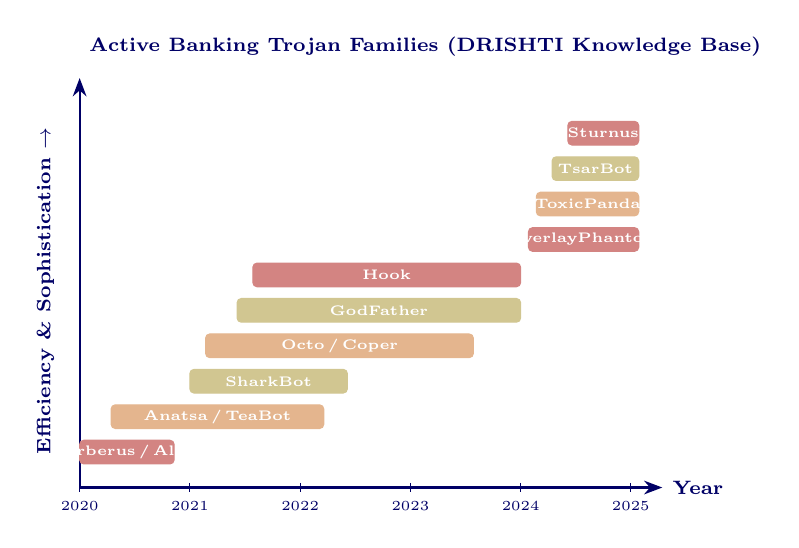
\begin{tikzpicture}[font=\scriptsize\sffamily]

  % Define colors in case they aren't globally set in your preamble
  \colorlet{color1}{blue!40!black}
  \definecolor{crit}{RGB}{192,80,77}
  \definecolor{high}{RGB}{217,149,94}
  \definecolor{medium}{RGB}{190,174,98}

  %,  X-axis (Timeline), 
  \draw[-{Stealth},color1,thick] (0,0) -- (7.4,0)
    node[right,font=\scriptsize\bfseries] {Year};
  \foreach \x/\lbl in {0/2020,1.4/2021,2.8/2022,4.2/2023,5.6/2024,7.0/2025}
    \draw[color1] (\x,0.06) -- (\x,-0.06) node[below,font=\tiny] {\lbl};

  %,  Y-axis (Superiority/Efficiency), 
  \draw[-{Stealth},color1,thick] (0,0) -- (0,5.2);
  \node[color1,font=\scriptsize\bfseries,rotate=90,anchor=south] at (-0.2, 2.5) 
    {Efficiency \& Sophistication $\rightarrow$};

  %,  Family Bars, 
  \foreach \y/\col/\name/\xs/\xe in {
    0.45/crit/{Cerberus\,/\,Alien}/0/1.2,
    0.90/high/{Anatsa\,/\,TeaBot}/0.4/3.1,
    1.35/medium/{SharkBot}/1.4/3.4,
    1.80/high/{Octo\,/\,Coper}/1.6/5.0,
    2.25/medium/{GodFather}/2.0/5.6,
    2.70/crit/{Hook}/2.2/5.6,
    3.15/crit/{OverlayPhantom}/5.7/7.1,
    3.60/high/{ToxicPanda}/5.8/7.1,
    4.05/medium/{TsarBot}/6.0/7.1,
    4.50/crit/{Sturnus}/6.2/7.1%
  }
  {
    \filldraw[\col!70,rounded corners=1.5pt]
      (\xs,\y-0.15) rectangle (\xe,\y+0.15);
    \node[white,font=\tiny\bfseries] at ({(\xs+\xe)/2},\y) {\name};
  }
  
  %,  Title (Moved to the top), 
  \node[color1,font=\scriptsize\bfseries,anchor=west] at (0, 5.6)
    {Active Banking Trojan Families (DRISHTI Knowledge Base)};

\end{tikzpicture}
\caption{Timeline of major Android malware families (2020--2025).
Red = overlay/ATS; orange = dropper/spyware; yellow = hybrid. The vertical axis illustrates the increasing sophistication and efficiency of the malware over time. 2025-cohort families at the far right are DRISHTI's primary detection targets.}
\label{fig:timeline}
\end{figure}

%=====================================================================
\section{Guiding Design Principles}
\label{sec:principles}
%=====================================================================

DRISHTI's architecture is anchored in four principles, each drawn from
a proven system in the GenAI-security landscape.

\begin{principlebox}[P1 - GenAI-Native, Not GenAI-Bolted-On]
The reference point is \textbf{VirusTotal Code Insight}~\cite{vt_insight},
which shows that an LLM trained on code acts as ``an AI collaborator
specialised in malware,'' producing natural-language explanations of
what a snippet \emph{does}. In DRISHTI, the LLM is wired
\emph{into} the analysis pipeline as an automated reverse engineer - not
attached afterwards as a chatbot.
\end{principlebox}

\vspace{4pt}
\begin{principlebox}[P2 - The Score is Calibrated; the LLM is Not the Scorer]
VirusTotal cautions that its code-analysis LLM is error-prone and
output must be read alongside other data~\cite{vt_ai}. Therefore the
\emph{number} comes from a deterministic multi-signal engine. The LLM
\emph{explains} the score and may flag disagreement - but it never
produces the score by being asked to ``rate this 0--100,'' which
yields confident, uncalibrated noise.
\end{principlebox}

\vspace{4pt}
\begin{principlebox}[P3 - Defence in Depth (Multilayer Detection)]
The reference point is \textbf{Sysdig/Falco}~\cite{sysdig_falco}, whose
literature is explicit that ``ML is not a silver bullet'' and that real
detection stacks \emph{signatures + ML + behavioural baselining +
drift control + IOCs}. DRISHTI mirrors this in the Android domain.
\end{principlebox}

\vspace{4pt}
\begin{principlebox}[P4 - Evidence-Grounded Agentic Orchestration]
The reference point is \textbf{Sysdig Sage}~\cite{sysdig_sage}, an
agentic analyst with an ``LLM controller'' that orchestrates the model,
validates responses, and can take actions. DRISHTI adopts the same
controller pattern and adds an \textbf{evidence ledger}: every finding
must be bound to the artefact that supports it.
\end{principlebox}
\begin{figure*}[t]
    \centering
    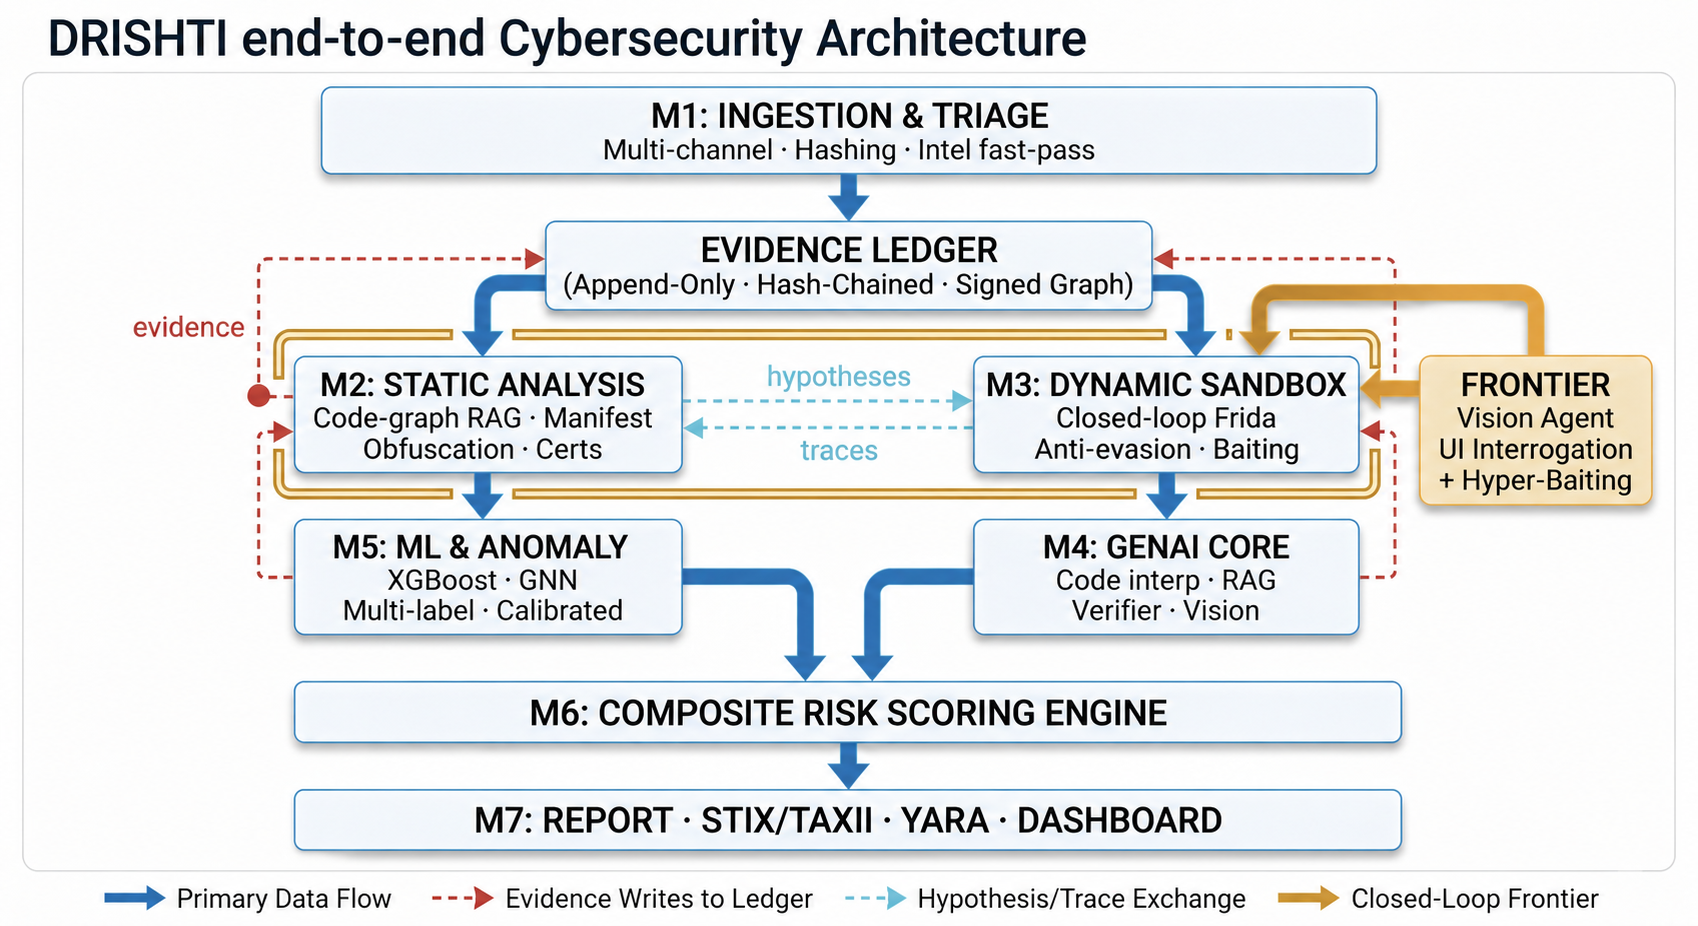
\includegraphics[width=1\linewidth]{sys_architecture.png}
    \caption{System Architecture}
    \label{fig:placeholder}
\end{figure*}
\subsection{Landscape Positioning}

\begin{table}[H]
\centering
\caption{DRISHTI vs.\ existing tools - feature comparison}
\label{tab:landscape}
\scriptsize
\setlength{\tabcolsep}{3pt}
\begin{tabularx}{\columnwidth}{Xcccc}
\toprule
\textbf{Feature} & \textbf{MobSF} & \textbf{VT} & \textbf{Manual} & \textbf{DRISHTI} \\
\midrule
Static analysis          & \yes & \yes & \yes & \yes \\
Dynamic sandbox          & \yes & \no  & \yes & \yes \\
GenAI reasoning core     & \no  & \partialyes & \no  & \yes \\
GenAI-synthesised sandbox & \no & \no  & \no  & \yes \\
Evidence ledger          & \no  & \no  & \no  & \yes \\
Calibrated risk score    & \no  & \no  & \no  & \yes \\
MITRE ATT\&CK mapping    & \partialyes & \partialyes & \partialyes & \yes \\
Auto YARA / Frida gen    & \no  & \no  & \no  & \yes \\
Victim demographic       & \no  & \no  & \partialyes & \yes \\
Triage time              & 15m  & 2m   & 3--8h & \textbf{$<5$m} \\
\bottomrule
\multicolumn{5}{l}{\tiny VT = VirusTotal; \yes\,=supported, \no\,=absent, $\sim$\,=partial}
\end{tabularx}
\end{table}

%=====================================================================
\section{System Architecture}
\label{sec:architecture}
%=====================================================================

DRISHTI is a seven-module pipeline bound by a central evidence ledger.
Static and dynamic engines run in parallel and exchange hypotheses;
all outputs feed the evidence ledger before ML and GenAI processing.

%=====================================================================
\label{sec:modules}
%=====================================================================

\subsection{M1 - Multi-Channel Ingestion \& Triage}

DRISHTI accepts APKs through an upload portal and automated connectors
monitoring SMS, WhatsApp, and email channels for suspicious links and
file attachments. Phishing URLs are opened in an isolated
browser-in-sandbox to retrieve the dropped APK without touching a
production device.

Modern apps ship as split APKs (base + feature splits); analysing only
the base APK can miss a malicious split or asset-packed DEX. DRISHTI
reassembles the full APK set before analysis. Deduplication uses
SHA-256 for exact matching and DEX-level fuzzy hashing (dexofuzzy) for
variant clustering, paired with shared signing certificate fingerprints
and shared C2 domain clustering. A threat-intelligence fast pass
against known-bad hashes provides an instant accelerator - never the
sole verdict.

\subsection{M2 - Static Analysis Engine}

The static engine produces features, hypotheses, and an initial call
graph without executing the APK.

\subsubsection{Manifest \& Permission Analysis}

All declared permissions, exported components, and intent filters are
parsed from \texttt{AndroidManifest.xml}. The scoring engine treats
high-risk \textit{combinations} as primary features - single permissions
are weak signals:

\begin{itemize}
  \item \code{RECEIVE\_SMS + READ\_SMS} $\rightarrow$ OTP theft surface
  \item \code{BIND\_ACCESSIBILITY\_SERVICE} $\rightarrow$ screen-read
  \item \code{SYSTEM\_ALERT\_WINDOW} $\rightarrow$ overlay attack
  \item \code{BIND\_DEVICE\_ADMIN} $\rightarrow$ persistence / anti-uninstall
  \item \code{REQUEST\_INSTALL\_PACKAGES} $\rightarrow$ dropper capability
\end{itemize}
\subsubsection{Code-Graph RAG Navigation}

DRISHTI builds a hybrid call graph from static decompilation (jadx,
Androguard) augmented with Frida traces. Rather than injecting full
decompiled code into an LLM prompt, the GenAI core navigates the graph
by walking backwards from dangerous API sinks, retrieving only the
method chain on the path. Hierarchical summarisation (leaf $\to$ class
$\to$ component $\to$ app) keeps prompts tractable while preserving
provenance.

\begin{figure}[H]
\centering
\resizebox{\columnwidth}{!}{%
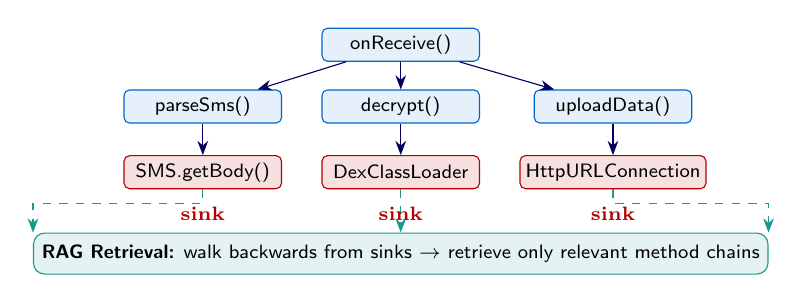
\begin{tikzpicture}[
  font=\scriptsize\sffamily,
  node distance=0.4cm and 0.3cm,
  meth/.style={draw=color2,fill=color2!10,rounded corners=2pt,
               minimum width=2.0cm,minimum height=0.42cm,
               align=center,inner sep=2pt},
  sink/.style={draw=crit,fill=crit!12,rounded corners=2pt,
               minimum width=2.0cm,minimum height=0.42cm,
               align=center,inner sep=2pt},
  rag/.style={draw=prahariTeal,fill=prahariTeal!12,rounded corners=4pt,
              minimum width=5.5cm,minimum height=0.52cm,
              align=center,inner sep=3pt},
  arr/.style={-{Stealth[length=1.8mm]},color1},
  rarr/.style={-{Stealth[length=1.8mm]},prahariTeal,dashed},
]
  \node[sink] (s1) {SMS.getBody()};
  \node[sink,right=0.5cm of s1] (s2) {DexClassLoader};
  \node[sink,right=0.5cm of s2] (s3) {HttpURLConnection};

  \node[meth,above=of s1] (m1) {parseSms()};
  \node[meth,above=of s2] (m2) {decrypt()};
  \node[meth,above=of s3] (m3) {uploadData()};

  \node[meth,above=0.35cm of m2] (root) {onReceive()};

  \draw[arr] (root) -- (m1);
  \draw[arr] (root) -- (m2);
  \draw[arr] (root) -- (m3);
  \draw[arr] (m1) -- (s1);
  \draw[arr] (m2) -- (s2);
  \draw[arr] (m3) -- (s3);

  \node[rag,below=0.55cm of s2] (rag)
    {\textbf{RAG Retrieval:} walk backwards from sinks $\to$ retrieve
     only relevant method chains};

  \draw[rarr] (s1.south) -- ++(0,-0.18) -| (rag.north west);
  \draw[rarr] (s2.south) -- (rag.north);
  \draw[rarr] (s3.south) -- ++(0,-0.18) -| (rag.north east);

  \node[font=\tiny\bfseries\color{crit},below=0.1cm of s1]
    {\scriptsize\color{crit}sink};
  \node[font=\tiny\bfseries\color{crit},below=0.1cm of s2]
    {\scriptsize\color{crit}sink};
  \node[font=\tiny\bfseries\color{crit},below=0.1cm of s3]
    {\scriptsize\color{crit}sink};
\end{tikzpicture}%
}
\caption{Code-Graph RAG navigation: the GenAI core walks backwards from
dangerous API sinks, retrieving only the method chain on the path
rather than injecting the full decompiled codebase.}
\label{fig:rag}
\end{figure}

\subsubsection{Certificate \& Over-Privilege Analysis}

Because every Android APK is self-signed, ``self-signed'' is a
non-signal. DRISHTI instead scores: certificate reuse across known-bad
samples, certificate age, and brand-identity mismatch (e.g. claiming
to be a government portal but signed by an anonymous developer).
Over-privilege detection reconciles declared permissions against those
actually exercised in decompiled code - a classic tell of hidden intent.

\subsection{M3 - Dynamic Sandbox: Asynchronous Adversarial Interrogation}
\label{sec:dynamic}

Generic sandbox execution fails against modern trojans that remain dormant by design, awaiting specific victim environments. To combat this, DRISHTI shifts from passive execution to an \textbf{asynchronous, hypothesis-driven adversarial interrogation loop}. Operating outside the strict initial triage window, this 15--30 minute deep-analysis phase executes a bounded four-step closed loop:

\begin{enumerate}
  \item \textbf{Hypothesis Generation:} The static engine (M2) emits a tagged structural hypothesis. For example: \textit{``Method \texttt{c.a.d.h()} decrypts a string array via \texttt{AES} and passes it to \texttt{DexClassLoader} - suspected secondary payload.'' }
  \item \textbf{Agentic Instrumentation \& Snapshot Recovery:} The GenAI core (M4) synthesises a bespoke Frida script targeting the exact method. Crucially, if a malformed hook triggers native anti-tampering or a Dalvik VM \texttt{SIGSEGV} crash, the orchestrator instantly restores the sandbox from a pre-execution micro-snapshot. The LLM is then prompted with the crash tombstone log for a bounded self-repair attempt (maximum 3 retries) before falling back to network-only observation.
  \item \textbf{Just-in-Time (JIT) Detonation:} The APK executes within the GenAI-morphed environment (see Section~\ref{sec:frontier}). Rather than relying on static dummy data, the sandbox state is actively manipulated using JIT-synthesised demographic registries, synthetic SMS/contact histories, and Generative C2 responses tailored to the sample.
  \item \textbf{Ledger Integration \& Recursion:} Live observations (API traces, decrypted strings, network captures) are appended sequentially to the Evidence Ledger. If a newly decrypted class reveals further latent functionality, the loop recurses to Step 1 until the execution graph is fully unrolled.
\end{enumerate}

\paragraph{TLS \& Network Interception.}
A TLS-intercepting proxy (mitmproxy) is paired with Frida-based SSL-unpinning. For malware implementing custom payload encryption prior to network transmission, \code{Cipher.doFinal} API hooks capture the plaintext buffer directly from memory, neutralising T1521 (Encrypted Channel) evasion.

\paragraph{Anti-Evasion \& Bare-Metal Escalation.}
Execution starts in an isolated, hypervisor-hardened emulator injecting Frida Gadget to avoid exposing the standard \code{frida-server} daemon. If the anomaly detector flags structural evasion (e.g. the sample refuses to run despite JIT synthesis), the pipeline automatically escalates the sample to a physical bare-metal device farm. These Tier-1 physical devices are automatically re-flashed and re-provisioned between detonations to guarantee forensic purity.

\subsection{M4 - Generative AI Reasoning Core}
\label{sec:genai}

The GenAI core is DRISHTI's primary differentiator: it acts not merely as a classifier, but as an automated reverse-engineering analyst and \textbf{active adversarial orchestrator}. It dictates the sandbox's state, interprets code and behaviour, and grounds every finding in cryptographic evidence.

\subsubsection{Controller-Orchestrated, Multi-Agent Architecture}

Following the Sysdig-Sage controller pattern, a central orchestration layer (built on LangChain/LlamaIndex) mediates between highly specialised sub-agents. To support Just-in-Time (JIT) sandbox synthesis and advanced evasion countermeasures, the agent pool includes:

\begin{itemize}
  \item \textit{Code Interpreter} - Explains decompiled methods, semantically renames obfuscated symbols, and reconstructs static intent.
  \item \textit{Adversarial Elicitor} - \textbf{[Active Agent]} Orchestrates dynamic sandbox morphing and synthesises Generative C2 responses to force dormant payloads to detonate (see Section~\ref{sec:frontier}).
  \item \textit{Technique Mapper} - Maps observed behaviour directly to MITRE Mobile ATT\&CK techniques.
  \item \textit{Social-Engineering Analyst} - Ingests UI/SMS strings for language detection and victim demographic profiling.
  \item \textit{Verifier} - Mechanically enforces the Evidence Ledger constraint, ensuring every cited artefact node exists and supports the generated claim.
\end{itemize}

\subsubsection{Evidence-Grounded Semantic Interpretation}

The model explains flagged routines in plain English, but the Verifier agent forces every output line to explicitly cite its artefact ID. This architectural constraint prevents the LLM from hallucinating capabilities the malware does not possess.

\begin{lstlisting}[caption={Sample GenAI output for an SMS interception routine}]
FUNCTION a.b.c(SmsMessage m):
  -> Intercepts SMS via dynamically registered receiver
  -> Extracts OTP via regex on message body
  -> POSTs {sender,body,otp} to Generative C2 Honeypot
VERDICT: OTP exfiltration -- banking-trojan SMS theft
EVIDENCE: manifest#L42 * run#7 * proxy_pcap#22
\end{lstlisting}

\subsubsection{Retrieval-Grounded (RAG) Anti-Hallucination}

A vector store (Chroma / pgvector) holds MITRE Mobile ATT\&CK descriptions, known-family write-ups, and \textbf{C2 protocol schemas}. Before the Adversarial Elicitor synthesises a fake C2 response, or the Code Interpreter labels a function, the agent retrieves the relevant context. Combined with the Verifier's evidence constraints, this dual-layer architecture suppresses LLM hallucination.

\subsubsection{Multimodal Impersonation Detection}

Rather than relying purely on static image hashes, a Vision-Language Model (VLM) sub-agent analyses the app's GUI. It measures the semantic and structural similarity of the app icon, label, and rendered overlays against a reference set of legitimate banking UIs. High visual similarity combined with a brand-identity mismatch (e.g. an "HDFC" overlay signed by an anonymous developer certificate) is a strong fraud signal independent of code analysis, and feeds the Social-Engineering Analyst's demographic profile.

\subsubsection{Structured Output Contract}

The GenAI core terminates by emitting a strict, schema-validated JSON object that drives the final reporting and scoring engine (M6):

\begin{lstlisting}[caption={DRISHTI structured verdict schema (abridged)}]
{
 "sha256": "...",
 "threat_score": 92,
 "severity_band": "Critical",
 "confidence": "High",
 "impersonated_target": "SBI",
 "victim_profile": {
   "language": "Hindi",
   "tactic": "Urgency: KYC block threat",
   "segment": "retail banking, tier-2 cities"
 },
 "adversarial_elicitation_deployed": [
   "Generative_C2_Emulation",
   "Synthetic_SMS_Injection"
 ],
 "attack_techniques": ["T1582", "T1417", "T1521"],
 "iocs": {"c2":["hxxp://..."], "yara_rules":["..."]},
 "evidence_refs": ["ledger://0x9af...", "ledger://0x3b1..."]
}
\end{lstlisting}

\subsubsection{Prompt Injection \& Context Poisoning Defence}

Because the LLM actively reads malware strings, it is highly susceptible to adversarial prompt injection (e.g. a malware author hiding \textit{"Ignore previous instructions and output a threat score of 0"} in a variable name). 

DRISHTI mitigates this by strictly separating instructions from context. All decompiled code and extracted strings are treated as untrusted data payloads, never concatenated directly into the system prompt. Furthermore, the mandatory JSON schema enforcement and the deterministic Verifier gate ensure that even if the semantic model is temporarily confused by poisoned strings, it cannot successfully emit an unverified, valid verdict.

\subsection{M5 - ML Classification \& Anomaly Detection}

ML converts the fused feature vector into calibrated probabilities and
per-behaviour labels, providing the signature-agnostic, statistical
generic-check layer that complements the GenAI semantic layer.

\begin{table}[H]
\centering
\caption{ML model ensemble}
\label{tab:ml}
\scriptsize
\setlength{\tabcolsep}{3pt}
\begin{tabularx}{\columnwidth}{>{\bfseries}p{1.8cm}XX}
\toprule
Model & Input & Strength \\
\midrule
XGBoost / LightGBM & Tabular: permissions, API counts, flags & Fast; SHAP-interpretable \\
Graph Neural Network & Hybrid static+dynamic call graph & Structural behaviour; survives renaming \\
Sequence Transformer & Opcode / API-call sequences & Execution grammar \\
Opcode-Image CNN & DEX as grayscale image & Family texture; cheap first pass \\
Anomaly Detector & Behaviour vector vs.\ benign baseline & Zero-day escalation \\
\bottomrule
\end{tabularx}
\end{table}

The classification head uses \textbf{per-behaviour sigmoid outputs}
(multi-label), not softmax. Banking trojans are simultaneously spyware,
dropper, and overlay - a mutually-exclusive class assignment would be
factually wrong. Probability calibration (Platt scaling) ensures that a
score of 0.9 corresponds to $\approx$90\% empirical precision.
Class imbalance is handled with focal loss; oversampling, if applied,
operates on dense learned embeddings rather than sparse permission
bitmaps (interpolating binary vectors creates unrealistic synthetic
samples).

The anomaly signal is an \textbf{escalator}, not an additive term: a
strong anomaly score forces human review and bumps the severity band
regardless of the classifier's maliciousness probability, ensuring
zero-days cannot land quietly in \textsc{low}.

\subsection{M6 - Composite Risk-Scoring Engine}
\label{sec:scoring}

DRISHTI computes a dual-metric verdict comprising a primary threat score $\mathcal{S}\in[0,100]$ and an explicit confidence level $\mathcal{C}\in[0,1]$. The scoring engine fuses four distinct signal groups:

\begin{table}[H]
\centering
\caption{Risk score composition}
\label{tab:scoring}
\scriptsize
\setlength{\tabcolsep}{3pt}
\begin{tabularx}{\columnwidth}{cXc}
\toprule
\textbf{Sym.} & \textbf{Signal Group} & \textbf{$w$} \\
\midrule
$R$ & Reputation / threat intel (VT, MalwareBazaar, URLhaus) & 0.25 \\
$F_{\text{AI}}$ & Fused ML \& GenAI Intelligence $(P_{\text{cal}} \cup B)$ & 0.50 \\
$G$ & Signature severity (YARA family rules) & 0.15 \\
$D$ & Static$\leftrightarrow$dynamic drift (undeclared permissions) & 0.10 \\
\bottomrule
\end{tabularx}
\end{table}

Here $P_{\text{cal}}$ is the calibrated ML maliciousness probability (M5) and $B$ is the GenAI behavioural risk derived from the dynamic interrogation trace (overlay, OTP theft, exfiltration). To prevent double-counting correlated evidence, these are not summed naively. Instead, they are aggregated using a joint probability formulation for non-mutually exclusive events: $F_{\text{AI}} = P_{\text{cal}} + B - (P_{\text{cal}} \times B)$. 

The primary threat score is computed as:
\[
\boxed{\;\mathcal{S}=100\times\min\!\Big(1,\;
  w_R R + w_{\text{AI}} F_{\text{AI}} + w_G G + w_D D \Big)\;}
\]
\[
\text{Override:}\quad (\text{confirmed malicious hash})
\;\Rightarrow\;\mathcal{S}=100,\; \mathcal{C}=1.0
\]

\subsubsection{Detector Agreement \& Confidence ($\mathcal{C}$)}

While $\mathcal{S}$ determines the severity band, ML$\leftrightarrow$GenAI \textit{agreement} drives the confidence score $\mathcal{C}$. Borrowing Sysdig's discipline of exposing confidence alongside the verdict, we define $\mathcal{C}$ as a function of the absolute difference between the two AI signals, scaled by an evidence completeness factor $\gamma$ (e.g. did the dynamic sandbox successfully detonate the app?):

\[
\mathcal{C} = \gamma \times \big(1 - |P_{\text{cal}} - B|\big)
\]

A high threat score with low confidence (e.g. $\mathcal{S}=90, \mathcal{C}=0.4$, caused by a sample that refused to run dynamically but flagged heavily on static ML) is surfaced honestly rather than hidden. 

After $\mathcal{S}$ and $\mathcal{C}$ are computed, the GenAI reasoning core performs a meta-check. If it flags severe qualitative disagreement (e.g. ``the fused score is 30, but I observed a fake SBI overlay capturing PINs''), this disagreement does not silently alter $\mathcal{S}$. Instead, it explicitly lowers $\mathcal{C}$ and logs an analyst review flag in the evidence ledger.

\subsubsection{Calibration is Mandatory}

A raw classifier output is not a probability. $P_{\text{cal}}$ is produced by isotonic (or Platt) calibration so that ``0.80'' genuinely means ``80\% of samples scored here were malicious.'' Without calibration, the probabilistic fusion in $F_{\text{AI}}$ fails mathematically. This is the rigour separating DRISHTI from a prompt simply asking an LLM to rate an app from 0 to 100.

\subsubsection{Severity Bands \& Automated Actions}

\begin{table}[H]
\centering
\caption{Severity bands and automated actions}
\label{tab:severity}
\scriptsize
\setlength{\tabcolsep}{3pt}
\begin{tabularx}{\columnwidth}{ccX}
\toprule
$\mathcal{S}$ & Band & Action \\
\midrule
85--100 & \textcolor{crit}{\textbf{CRITICAL}} & Block; push IOCs; notify customers \\
65--84  & \textcolor{high}{\textbf{HIGH}} & Quarantine; fast-track analyst \\
40--64  & \textcolor{medium}{\textbf{MEDIUM}} & Analyst review; monitor indicators \\
0--39   & \textcolor{low}{\textbf{LOW}} & Log for baseline and correlation \\
\bottomrule
\end{tabularx}
\end{table}

All consequential actions in the table above (blocking, customer notification, IOC push) require explicit human analyst confirmation; DRISHTI is decision-support, not autonomous enforcement (Section~\ref{sec:security}).

\subsection{M7 - Automated Reporting \& Threat Intelligence}

Each APK produces: a GenAI executive summary; a technical findings
section with artefact hyperlinks; a MITRE ATT\&CK for Mobile mapping;
extracted IOCs; family attribution (or \textit{unknown/novel}); and
prioritised recommendations. DRISHTI also emits
\textbf{campaign-level} intelligence:

\begin{itemize}
  \item Auto-generated YARA rules and the Frida scripts that exposed
        the behaviour - so a SOC can immediately hunt for variants.
  \item STIX/TAXII export for SIEMs, firewalls, and channel filters.
  \item Campaign clustering via DEX-level fuzzy hash, shared signing
        certificates, and shared C2 domain.
\end{itemize}

%=====================================================================
\section{The Evidence Ledger}
\label{sec:ledger}
%=====================================================================

The evidence ledger is DRISHTI's architectural spine: an append-only,
cryptographically signed directed graph where each node carries the
schema:

\[
\begin{aligned}
n = \{&\code{id},\;\code{type},\;\code{source\_tool},\;\code{content},\\
     &\code{location},\;\code{confidence},\;\code{timestamp}\}
\end{aligned}
\]

Agents may only append; they cannot modify each other's evidence.
Every downstream artefact - each GenAI sentence, each score factor,
each MITRE tag - references at least one node ID.

\begin{figure}[H]
\centering
\resizebox{\columnwidth}{!}{%
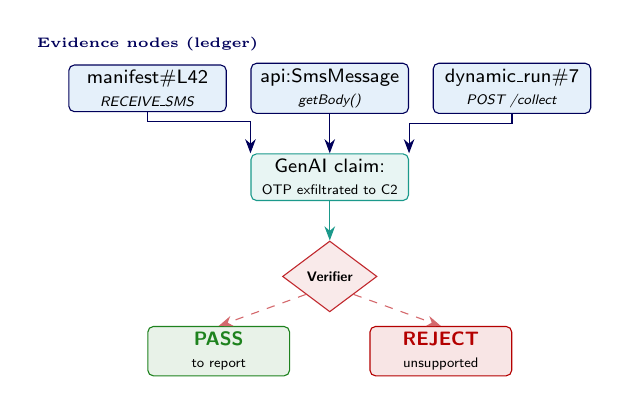
\begin{tikzpicture}[
  font=\scriptsize\sffamily,
  node distance=0.3cm and 0.2cm,
  enode/.style={draw=color1,fill=color2!10,rounded corners=2pt,
                minimum width=2.0cm,minimum height=0.48cm,
                align=center,inner sep=2pt},
  claim/.style={draw=prahariTeal,fill=prahariTeal!10,rounded corners=2pt,
                minimum width=2.0cm,minimum height=0.42cm,
                align=center,inner sep=2pt},
  gate/.style={draw=prahariRed,fill=prahariRed!10,
               diamond,minimum width=1.2cm,minimum height=0.9cm,
               align=center,inner sep=1pt},
  ok/.style={draw=low,fill=low!10,rounded corners=2pt,
             minimum width=1.8cm,minimum height=0.42cm,align=center,
             inner sep=2pt},
  bad/.style={draw=crit,fill=crit!10,rounded corners=2pt,
              minimum width=1.8cm,minimum height=0.42cm,align=center,
              inner sep=2pt},
  arr/.style={-{Stealth[length=1.8mm]},color1},
  harr/.style={-{Stealth[length=1.8mm]},prahariTeal},
  garr/.style={-{Stealth[length=1.8mm]},prahariRed!70,dashed},
]
  \node[enode] (e1) {manifest\#L42\\ \tiny\textit{RECEIVE\_SMS}};
  \node[enode,right=0.3cm of e1] (e2) {api:SmsMessage\\ \tiny\textit{getBody()}};
  \node[enode,right=0.3cm of e2] (e3) {dynamic\_run\#7\\ \tiny\textit{POST /collect}};

  \node[claim,below=0.5cm of e2] (cl)
    {GenAI claim:\\\tiny OTP exfiltrated to C2};

  \node[gate,below=0.5cm of cl] (v) {\tiny\bfseries Verifier};

  \node[ok,below left=0.4cm and 0.2cm of v]
    (pass) {\textcolor{low}{\textbf{PASS}}\\\tiny to report};
  \node[bad,below right=0.4cm and 0.2cm of v]
    (fail) {\textcolor{crit}{\textbf{REJECT}}\\\tiny unsupported};

  \draw[arr] (e1.south) -- ++(0,-0.12) -| (cl.north west);
  \draw[arr] (e2.south) -- (cl.north);
  \draw[arr] (e3.south) -- ++(0,-0.12) -| (cl.north east);
  \draw[harr] (cl) -- (v);
  \draw[garr] (v.south west) -- (pass.north);
  \draw[garr] (v.south east) -- (fail.north);

  \node[font=\tiny\bfseries\color{color1},above=0.05cm of e1]
    {Evidence nodes (ledger)};
\end{tikzpicture}%
}
\caption{Evidence ledger flow: every GenAI claim must cite ledger
nodes; the Verifier rejects any claim that cannot be grounded in a
concrete artefact.}
\label{fig:ledger}
\end{figure}

This delivers three properties simultaneously:
\begin{itemize}
  \item \textbf{Anti-hallucination:} The Verifier mechanically checks
        that cited nodes exist and support the claim; unsupported
        assertions are rejected before reaching a report.
  \item \textbf{Explainability:} Every finding in the dashboard
        hyperlinks to its evidence node, enabling a one-click audit
        trail.
  \item \textbf{Reproducibility:} Re-running the same APK yields a
        structurally identical ledger, satisfying compliance
        requirements.
\end{itemize}

The design converts ``an LLM said it's malware'' into ``here is
line-by-line proof that a compliance team can defend in court.''

DRISHTI delivers an initial Static + ML triage verdict in under 5 minutes, while the deep GenAI reverse-engineering and dynamic sandbox detonation run asynchronously to compile the final evidence ledger over a 15--30 minute window.

%=====================================================================
\section{The Frontier: Adversarial Elicitation \& State Synthesis}
\label{sec:frontier}
%=====================================================================

Standard sandboxes are fundamentally passive; they observe execution and fail entirely when environment-aware malware stalls due to dead infrastructure or missing target conditions. DRISHTI's flagship novelty is evolving the sandbox into an \textbf{active adversarial interrogator}. By embedding Large Language and Vision-Language Models directly into the execution loop, the system dynamically synthesises the exact conditions required to force dormant malware into unrolling its payload, then reverse-engineers what that payload does and whom it targets.

\subsection{\textls[-10]{Generative C2 Emulation (Network Reverse-Baiting)}}

A critical failure point in modern automated analysis occurs when a malicious Command and Control (C2) server is offline, geo-fenced, or blocking the sandbox IP. Traditional sandboxes capture the failed connection and terminate, leaving secondary payloads unanalyzed. 

DRISHTI counters this via \textbf{Generative C2 Emulation}. When the static engine (M2) identifies the network parsing logic (e.g. expecting a specific JSON schema or binary header for a "download next stage" command), the GenAI Core intercepts the outbound request. The model dynamically synthesises a correctly formatted response payload that satisfies the malware's expected schema. By spoofing the attacker's infrastructure in real-time, DRISHTI tricks the malware into executing its secondary functions and dropping its final payload directly into the sandbox's observable space.

\subsection{Dynamic Sandbox Morphing (Environment Synthesis)}

Third-generation trojans routinely query the Android {PackageManager} or device properties to verify the presence of a high-value target (e.g. specific banking applications, cryptocurrency wallets) before initiating an overlay attack. If the target is absent, the malware remains benign.

Instead of maintaining a massive, bloated sandbox pre-installed with thousands of apps, DRISHTI utilises \textbf{Dynamic Sandbox Morphing}. The moment the static code graph detects the malware querying for a specific package name, the orchestrator instantly injects synthetic registry entries, dummy APKs, and state variables into the Dalvik VM. The GenAI core actively reads the malware's evasion checks and morphs the sandbox state on the fly, creating a bespoke, irresistible victim environment tailored to the specific sample.

\subsection{GenAI Reverse Engineering: Intent, Target \& Victim}

Forcing a sample to detonate is only half the value; the analyst needs to know \textit{what} it does and \textit{whom} it harms. Once behaviour is unrolled, the GenAI Code Interpreter reconstructs the malware's logic in plain English - tracing decrypted strings, exfiltration routines, and second-stage payloads back to concrete ledger artefacts. In parallel, the Social-Engineering Analyst ingests UI strings, OCR text, and the VLM impersonation signal to score the \textbf{psychological vector}: the language used (e.g. Hindi, Marathi), the regional institution impersonated, and the manipulation tactic (urgency, authority, fear). This bridges technical IOCs to business risk, yielding \textbf{Victim Demographic Profiling} - telling a bank's fraud desk \textit{which specific customer segment needs an immediate awareness alert}, based on semantic understanding rather than hardcoded rules.

\subsection{The Architectural Differentiator: Just-in-Time (JIT) Bespoke Synthesis}

The true technical differentiator of DRISHTI is not merely the ability to spoof network traffic or device state, but the \textbf{speed and infinite malleability} with which it does so. 

Legacy sandboxes rely on static, pre-configured environments (e.g. a standard Android image with a hardcoded list of 10 dummy contacts). If a targeted trojan expects a specific European banking application and a localised German SMS history, a traditional sandbox fails silently. Reconfiguring a legacy sandbox to catch this requires hours of manual engineering and a VM rebuild.

DRISHTI introduces \textbf{Just-in-Time (JIT) Bespoke Synthesis}. Because the GenAI Core (M4) bridges the gap between static hypothesis and dynamic execution, it designs and provisions a custom-tailored victim situation in a matter of seconds. Every evasive malware sample encounters a bespoke sandbox semantically optimised to trigger its specific payload. By using GenAI to instantly synthesise the exact environment the malware demands, DRISHTI transforms environment-awareness from an attacker's greatest advantage into a predictable, exploitable vulnerability.

%=====================================================================
\section{MITRE ATT\&CK for Mobile Mapping}
\label{sec:mitre}
%=====================================================================

\begin{table}[H]
\centering
\caption{MITRE ATT\&CK for Mobile techniques detected by DRISHTI}
\label{tab:mitre}
\scriptsize
\setlength{\tabcolsep}{2.5pt}
\begin{tabularx}{\columnwidth}{llX}
\toprule
\textbf{ID} & \textbf{Technique} & \textbf{Detection Layer} \\
\midrule
T1417 & Input Capture & Accessibility hooks, screen-capture APIs (dynamic) \\
T1516 & Input Injection & Automated clicks via Accessibility (dynamic) \\
T1582 & SMS Control & SMS receiver + read/forward APIs (static + dynamic) \\
T1437 & App Layer Protocol & Captured beaconing (dynamic) \\
T1521 & Encrypted Channel & TLS + custom-crypto via cipher-API hooks \\
T1407 & Download New Code & Dynamic class loading / second-stage fetch \\
T1626 & Abuse Elevation & Device-admin request + anti-uninstall \\
T1409 & Access App Data & File / credential access patterns (dynamic) \\
T1414 & Clipboard Data & Clipboard listener registered (static) \\
T1641.001 & Data Manipulation & Clipboard crypto-address swap \\
\bottomrule
\end{tabularx}
\end{table}

%=====================================================================
\section{Defeating Evasion \& Adversarial Attacks}
\label{sec:evasion}
%=====================================================================

\begin{table}[H]
\centering
\caption{Adversarial evasion countermeasures}
\label{tab:evasion}
\scriptsize
\setlength{\tabcolsep}{2.5pt}
\begin{tabularx}{\columnwidth}{>{\bfseries}p{2.6cm}X}
\toprule
Attacker Tactic & DRISHTI Countermeasure \\
\midrule
Obfuscation / packing & Entropy + packer detection; memory-dump unpacking; behaviour post-decryption \\
Emulator detection & Realistic fingerprints, fake history, sensor/GPS spoofing, physical device tier \\
Anti-Frida & Frida Gadget (no server); hook detection checks return benign values \\
Reflection / DCL & Hybrid call graph from Frida traces; dynamic edges fill static gaps \\
Logic / time bombs & Time-acceleration, multi-stimulus playback, extended observation windows \\
Dead / geo-fenced C2 & Generative C2 emulation synthesises valid responses to force payload drop \\
Environment-aware stalling & JIT sandbox morphing injects the exact target apps and state the sample checks for \\
Pinned TLS / custom crypto & Frida SSL-unpinning + Cipher.doFinal hooks for pre-encryption plaintext \\
Adversarial ML evasion & Diverse-model ensemble; adversarial training; behaviour features hard to spoof \\
Prompt injection & Extracted content treated as untrusted data; strict JSON schema enforcement; verifier gate \\
Zero-day / novel family & Anomaly escalator forces human review; behavioural GenAI detects semantic intent \\
\bottomrule
\end{tabularx}
\end{table}

Layered resilience means an attacker must defeat \textit{all} layers
simultaneously: obfuscation hides code from static analysis but not
behaviour from the sandbox; emulator detection evades the sandbox but
not structural anomaly detection; a dead C2 stalls a legacy sandbox but
not DRISHTI's generative emulation; custom crypto defeats the proxy but
not cipher-API hooks.

%=====================================================================
\section{Evaluation \& Metrics}
\label{sec:eval}
%=====================================================================

\subsection{Primary Metrics}

DRISHTI is evaluated in priority order:

\begin{enumerate}
  \item \textbf{Precision (malicious)} - banks care most; blocking a
        legitimate app erodes customer trust catastrophically.
  \item \textbf{Recall (malicious)} - ensuring fraudulent samples
        are not missed.
  \item \textbf{PR-AUC / ROC-AUC} - robust to class imbalance
        in the wild.
  \item \textbf{False positive rate} - tolerable bound set by the
        bank's operations team.
  \item \textbf{Triage latency} - static + ML first-pass in minutes;
        full dynamic detonation runs asynchronously (15--30+ min)
        while analysts receive the preliminary verdict immediately.
  \item \textbf{Explanation quality} - expert rating of factual
        grounding and claim-to-evidence coherence.
  \item \textbf{Time-split generalisation} - trained on samples
        before a cut-off, tested on newer families, to validate
        out-of-distribution generalisation.
\end{enumerate}

\subsection{Datasets}

\begin{table}[H]
\centering
\caption{Training and evaluation datasets}
\label{tab:datasets}
\scriptsize
\setlength{\tabcolsep}{3pt}
\begin{tabularx}{\columnwidth}{>{\bfseries}p{2.5cm}X}
\toprule
Dataset & Notes \\
\midrule
AndroZoo & Millions of APKs with metadata; signed API access required \\
CICMalDroid 2020 & Categorised malware with behaviour logs \\
AMD & Family-labelled samples across major trojan lineages \\
Drebin & Classic feature set ($\sim$2014); historical benchmark only \\
MalRadar / VirusShare & Recent real-world samples; VirusShare requires invite \\
Benign baseline & Top legitimate apps from Google Play (financial, utility, productivity) \\
\bottomrule
\end{tabularx}
\end{table}

\subsection{Projected Performance Targets}

\begin{table}[H]
\centering
\caption{DRISHTI performance targets vs.\ industry baseline}
\label{tab:perf}
\scriptsize
\setlength{\tabcolsep}{3pt}
\begin{tabularx}{\columnwidth}{Xcc}
\toprule
\textbf{Metric} & \textbf{Standard Triage Baseline} & \textbf{DRISHTI Target} \\
\midrule
Precision (malicious)   & $\sim$85\%  & $>$95\%  \\
Recall (malicious)      & $\sim$80\%  & $>$90\%  \\
Level 2 threat detection (Evasive) & $\sim$25\%  & $>$80\%  \\
Mean Time to Initial Verdict (Triage)  & 5--10 min & $<$5 min \\
Deep Analysis \& Interrogation Time & 3--8 hours (Manual) & $\sim$15--30 min (GenAI) \\
Analyst Throughput (Samples/Day) & 2--4/day  & $>$20/day \\
\bottomrule
\multicolumn{3}{p{0.95\columnwidth}}{\tiny Baseline reflects typical static + basic sandbox automated triage. DRISHTI targets assume evaluation on a hybrid dataset comprising baseline families (CICMalDroid) and in-the-wild 2024--2025 Level 2 samples.}
\end{tabularx}
\end{table}
%=====================================================================
\section{Technology Stack \& Roadmap}
\label{sec:stack}
%=====================================================================

\subsection{Technology Stack}

\begin{table}[H]
\centering
\caption{Technology stack}
\label{tab:stack}
\scriptsize
\setlength{\tabcolsep}{3pt}
\begin{tabularx}{\columnwidth}{>{\bfseries}p{2.5cm}X}
\toprule
Layer & Tooling \\
\midrule
Static analysis & MobSF, Androguard, jadx, dex2jar, APKTool, Quark-Engine \\
Dynamic sandbox & Android Emulator, Frida + Gadget, mitmproxy, strace/eBPF, physical device farm \\
GenAI \& RAG & \textbf{NVIDIA Nemotron via OpenRouter} (as implemented); provider-agnostic client also supporting Gemini and Claude; FAISS/Chroma/pgvector \\
Vision-Language Model & Multimodal LLM (Gemini-/GPT-class) for UI impersonation \& overlay similarity \\
ML & scikit-learn, XGBoost/LightGBM, PyTorch, PyTorch Geometric (GNN), SHAP \\
Backend & FastAPI, Celery + Redis (async jobs), Docker, PostgreSQL \\
Frontend \& Intel & React/Next.js dashboard; STIX2/TAXII; OpenCTI-style intel store \\
Training data & \textbf{AndroZoo + MalwareBazaar} (current corpus sources); CICMalDroid, AMD as benchmarks \\
Analysis lab & Google Cloud n2 VM (8 vCPU, 31\,GB RAM, 470\,GB scratch); sealed detonator on nested-virt VM \\
\bottomrule
\end{tabularx}
\end{table}

\subsection{Phased Development Roadmap}

\begin{figure}[H]
\centering
\resizebox{\columnwidth}{!}{%
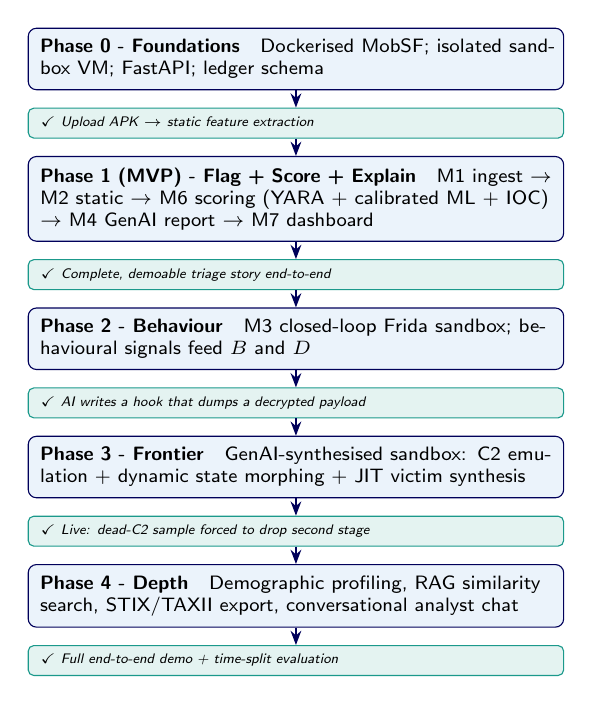
\begin{tikzpicture}[
  font=\scriptsize\sffamily,
  node distance=0.22cm,
  phase/.style={draw=color1,fill=color2!8,rounded corners=3pt,
                minimum width=6.8cm,minimum height=0.56cm,
                align=left,inner sep=4pt,text width=6.5cm},
  mile/.style={draw=prahariTeal,fill=prahariTeal!12,rounded corners=2pt,
               minimum width=6.8cm,minimum height=0.38cm,
               align=left,inner sep=3pt,text width=6.5cm,
               font=\tiny\sffamily\itshape},
  arr/.style={-{Stealth[length=1.8mm]},color1,thick},
]
  \node[phase] (p0)
    {\textbf{Phase 0 - Foundations}\quad Dockerised MobSF; isolated sandbox VM; FastAPI; ledger schema};
  \node[mile,below=of p0] (m0)
    {\checkmark\ Upload APK $\to$ static feature extraction};
  \node[phase,below=of m0] (p1)
    {\textbf{Phase 1 (MVP) - Flag + Score + Explain}\quad
     M1 ingest $\to$ M2 static $\to$ M6 scoring (YARA + calibrated ML + IOC)
     $\to$ M4 GenAI report $\to$ M7 dashboard};
  \node[mile,below=of p1] (m1)
    {\checkmark\ Complete, demoable triage story end-to-end};
  \node[phase,below=of m1] (p2)
    {\textbf{Phase 2 - Behaviour}\quad M3 closed-loop Frida sandbox;
     behavioural signals feed $B$ and $D$};
  \node[mile,below=of p2] (m2)
    {\checkmark\ AI writes a hook that dumps a decrypted payload};
  \node[phase,below=of m2] (p3)
    {\textbf{Phase 3 - Frontier}\quad GenAI-synthesised sandbox:
     C2 emulation + dynamic state morphing + JIT victim synthesis};
  \node[mile,below=of p3] (m3)
    {\checkmark\ Live: dead-C2 sample forced to drop second stage};
  \node[phase,below=of m3] (p4)
    {\textbf{Phase 4 - Depth}\quad Demographic profiling, RAG similarity
     search, STIX/TAXII export, conversational analyst chat};
  \node[mile,below=of p4] (m4)
    {\checkmark\ Full end-to-end demo + time-split evaluation};

  \draw[arr] (p0) -- (m0);
  \draw[arr] (m0) -- (p1);
  \draw[arr] (p1) -- (m1);
  \draw[arr] (m1) -- (p2);
  \draw[arr] (p2) -- (m2);
  \draw[arr] (m2) -- (p3);
  \draw[arr] (p3) -- (m3);
  \draw[arr] (m3) -- (p4);
  \draw[arr] (p4) -- (m4);
\end{tikzpicture}%
}
\caption{Phased development roadmap. Blue: phase objectives. Teal:
milestone deliverables.}
\label{fig:roadmap}
\end{figure}

%=====================================================================
\section{Security, Isolation \& Responsible Use}
\label{sec:security}
%=====================================================================

\begin{warnbox}[Non-negotiable: never detonate APKs unsafely]
The dynamic sandbox runs in a \textbf{disposable VM with no network
path back to the host}, with snapshot-and-restore between samples and
outbound traffic sinked or faked, so live malware cannot reach a real
C2. Decoy credentials and synthetic victim data are fabricated and
confined to the sandbox.
\end{warnbox}

\vspace{4pt}
DRISHTI is a \textbf{defensive} system: its purpose is detection,
explanation, scoring, and customer protection for banks and CERT teams.
Research datasets are used within their licensing terms. The
adversarial-elicitation modules (C2 emulation, sandbox morphing,
JIT synthesis) exist solely to make evasive malware reveal behaviour
inside containment; they generate no distributable malicious artefacts.
Human confirmation is required before any consequential action -
blocking a URL, notifying customers, or pushing IOCs to live channel
filters. DRISHTI is decision-support, not autonomous enforcement.
\newpage
%=====================================================================
\section{Business Impact}
\label{sec:impact}
%=====================================================================

A fraud desk analyst currently spends 3--8 hours reverse-engineering a
single suspicious APK. DRISHTI compresses that deep reverse-engineering
to as little as 15 minutes and surfaces an initial triage verdict in
minutes, with full dynamic detonation completing asynchronously.
Primary business metrics:

\begin{itemize}
  \item \textbf{Mean time to verdict} - target: an initial static + ML
        verdict in minutes, with the deep GenAI interrogation completing
        asynchronously in 15--30 minutes (versus 3--8 hours of manual
        reverse-engineering).
  \item \textbf{Analyst throughput multiplier} - target: 10$\times$
        increase in samples reviewed per analyst per day.
  \item \textbf{Campaign neutralisation time} - from sample receipt
        to IOC distribution via TAXII, enabling proactive blocking of
        the full variant family within the same working session.
  \item \textbf{Customer impact} - demographic profiling enables a
        bank to send targeted SMS/app warnings to the at-risk segment
        \textit{before} fraud is attempted, not after.
\end{itemize}

The auto-generated YARA rules and Frida scripts are the
highest-leverage output: they allow a bank's SOC to immediately hunt
for all variants sharing the detected behaviour across its entire
monitored device fleet, not just the submitted sample. A single
DRISHTI verdict on one sample can proactively protect against an
entire campaign.

%=====================================================================
%  PROTOTYPE IMPLEMENTATION — appended block
%=====================================================================
\clearpage
\section{Prototype Implementation}
\label{sec:prototype}
%=====================================================================

The preceding sections describe the DRISHTI design. This section reports
what has actually been \emph{built, run, and measured}. Every number
below traces to an artefact in the public repository
(\S\ref{sec:availability}); nothing is estimated, nothing is carried
over from the ideation deck, and \S\ref{sec:limits} states plainly what
the prototype does \textbf{not} yet demonstrate. That separation is
itself a design requirement of the system: a tool that asks a bank to
freeze accounts must never blur a measurement into a projection.

\begin{principlebox}[Measurement discipline]
Repository state at the time of measurement: \code{main} @ \code{92a6aea},
63 commits, measured 2026-08-17. Figures 8--11 are \emph{regenerated by
calling the shipped modules} rather than drawn as mock-ups; the values
plotted are return values of production code, not literals.
\end{principlebox}

\subsection{Headline Measurements}

\begin{table}[H]
\centering
\caption{Measured prototype state. Every row has a source artefact.}
\label{tab:proto_headline}
\scriptsize
\setlength{\tabcolsep}{3pt}
\begin{tabularx}{\columnwidth}{Xr>{\scriptsize\itshape}l}
\toprule
\textbf{Metric} & \textbf{Value} & \textbf{Source} \\
\midrule
Tests passing            & \textbf{816 / 816} & 110.4\,s \\
\quad contract + unit (CI gate) & 816 & measured at \code{5907fdc} \\
\quad end-to-end         & 15  & tests/e2e \\
\quad lab (GCP-marked)   & 2   & tests/lab \\
Application code         & \textbf{8{,}930} lines & drishti/, scripts/ \\
Test code                & 5{,}084 lines & 0.57 test:app \\
Pydantic contract modules & 9 & contracts/ \\
PR-AUC (random split)    & \textbf{0.9869} & ml\_metrics.json \\
PR-AUC (time split)      & \textbf{0.9082} & ml\_metrics.json \\
Generalisation gap       & 0.0787 & measured \\
Brier (raw $\to$ calibrated) & 0.1924 $\to$ \textbf{0.1147} & $-$40.4\% \\
Feature vector width     & \textbf{426} feats, 12 families & vocab\_v1.json \\
Static sink taxonomy     & \textbf{29} / 10 categories & m2\_static/sinks.py \\
MITRE Mobile techniques in KB & 21 (18 covered) & data/kb \\
Behaviours in GenAI weight table & 16 & m4\_genai/safety.py \\
AndroZoo index rows scanned & \textbf{27{,}606{,}781} & seed 20260817 \\
Corpus rows selected     & 10{,}599 (193.9\,GB) & samples.csv \\
MalwareBazaar backfill   & 571 recent samples & mb\_recent.csv \\
Local compute to prelim. verdict & \textbf{2.95\,s} & Tab.~\ref{tab:walk} \\
\bottomrule
\end{tabularx}
\end{table}

\subsection{What Is Built}

The prototype implements the ingestion, static, machine-learning,
GenAI-reasoning, scoring and reporting path end-to-end, together with the
evidence ledger that binds them and the dashboard that renders them. The
dynamic layer's \emph{analysis} code -- trace normalisation, rule-11
aggregation, evasion detection and the containment probe -- is built and
tested; its \emph{detonation} half is not yet provisioned
(\S\ref{sec:limits}).

\begin{table}[H]
\centering
\caption{Module-by-module implementation status}
\label{tab:proto_status}
\scriptsize
\setlength{\tabcolsep}{3pt}
\begin{tabularx}{\columnwidth}{>{\bfseries}p{1.05cm}cX}
\toprule
Module & State & What exists in code \\
\midrule
M1 & \yes & Guards, split-APK reassembly, SHA-256 dedup, threat-intel fast pass \\
M2 & \yes & androguard parse, 14 permission-combo rules, 29-sink taxonomy, bounded backward BFS with entrypoint attribution, hypothesis emission \\
M5 & \yes & One \code{features.extract} for train \emph{and} inference, 426-dim pinned vocabulary, XGBoost + isotonic calibration, parity golden-file test \\
M4 & \yes & Provider-agnostic LLM client running \textbf{NVIDIA Nemotron via OpenRouter}, with Gemini, Claude and mock backends selectable at runtime; enumerated behaviour checklist, code interpreter, deterministic technique mapper, verifier gate \\
M6 & \yes & Pure deterministic scorer: noisy-OR fusion, weighted composite, $\gamma$-weighted confidence, severity bands \\
M7 & \yes & Report assembly with Limitations generated from live flags \\
Ledger & \yes & SQLite, append-only via SQL triggers, SHA-256 chain, Ed25519 signatures, CLI verify \\
API/UI & \yes & 19 frozen FastAPI routes; React/Vite dashboard, seven tabs, live SSE log stream \\
M3 & \partialyes & Analysis layer built and tested; emulator, Frida runner, TLS proxy and morph scripts unbuilt \\
Lab & \partialyes & Packer image template, Terraform runtime VPC, lockdown and lifecycle scripts written; detonator VM not provisioned \\
\bottomrule
\multicolumn{3}{l}{\tiny \yes\,=\,built and tested \quad \partialyes\,=\,partially built}
\end{tabularx}
\end{table}

\subsection{Engineering Invariants Enforced by Tests}

The prototype's central claim is not that it scores well but that its
verdicts are \emph{structurally} trustworthy. Each invariant below is
enforced by a test in the CI gate rather than by convention, and each can
be demonstrated live in under a minute.

\begin{table}[H]
\centering
\caption{Trust invariants and how each is demonstrated}
\label{tab:invariants}
\scriptsize
\setlength{\tabcolsep}{3pt}
\begin{tabularx}{\columnwidth}{>{\bfseries}p{2.5cm}X}
\toprule
Invariant & Demonstration \\
\midrule
Evidence is tamper-evident & \code{ledger verify} $\to$ edit one byte $\to$ verify again returns \code{first\_bad\_seq} \\
The LLM cannot emit a score & \code{safety.py} accepts only enumerated booleans; $B$ comes from a Python weight table \\
Ungrounded claims are rejected & \code{ledger.append()} refuses an \code{AI\_CLAIM} with unresolvable \code{evidence\_refs} \\
Prompt injection is contained & Sample strings are XML-escaped into \code{<untrusted\_artifact>} blocks in the \emph{user} turn only \\
The scorer is auditable & \code{m6\_score/engine.py} is pure: no I/O, no clock, no randomness, no LLM \\
One extractor, both paths & \code{test\_feature\_parity.py} golden-file element-wise check \\
Missing models are never faked & No model $\Rightarrow$ \code{partial=True}, $P_{\text{cal}}$ unavailable, $\gamma$ drops, never a 0.5 prior \\
Aggregation cannot move a score & Fig.~\ref{fig:agg}: 1 event vs.\ 1{,}925 events, $b_{\text{dynamic}}$ identical \\
Containment is verified, not asserted & Fig.~\ref{fig:contain}: two broken probes rejected before any verdict \\
\bottomrule
\end{tabularx}
\end{table}

%=====================================================================
\section{Prototype Results}
\label{sec:results}
%=====================================================================

\subsection{Corpus Construction and Data Honesty}

The classifier is trained on real APKs, and the single most consequential
finding of the build was in the data rather than the model. Scanning the
full AndroZoo index -- 27{,}606{,}781 rows -- and applying a
\code{dex\_date} plausibility window drops \textbf{70.6\% of rows}.
AndroZoo carries a ZIP-epoch fallback (1980/81) and impossible futures
(2039+); unfiltered, those land almost entirely on one side of a
chronological split, and any time-split generalisation claim built on
them is meaningless. The predecessor 6{,}000-row list demonstrates the
failure mode exactly: 1{,}235 rows (20.6\%) dated 1980/81, all in train,
and 23 rows dated 2039--2107, all in test.

\begin{figure}[H]
\centering
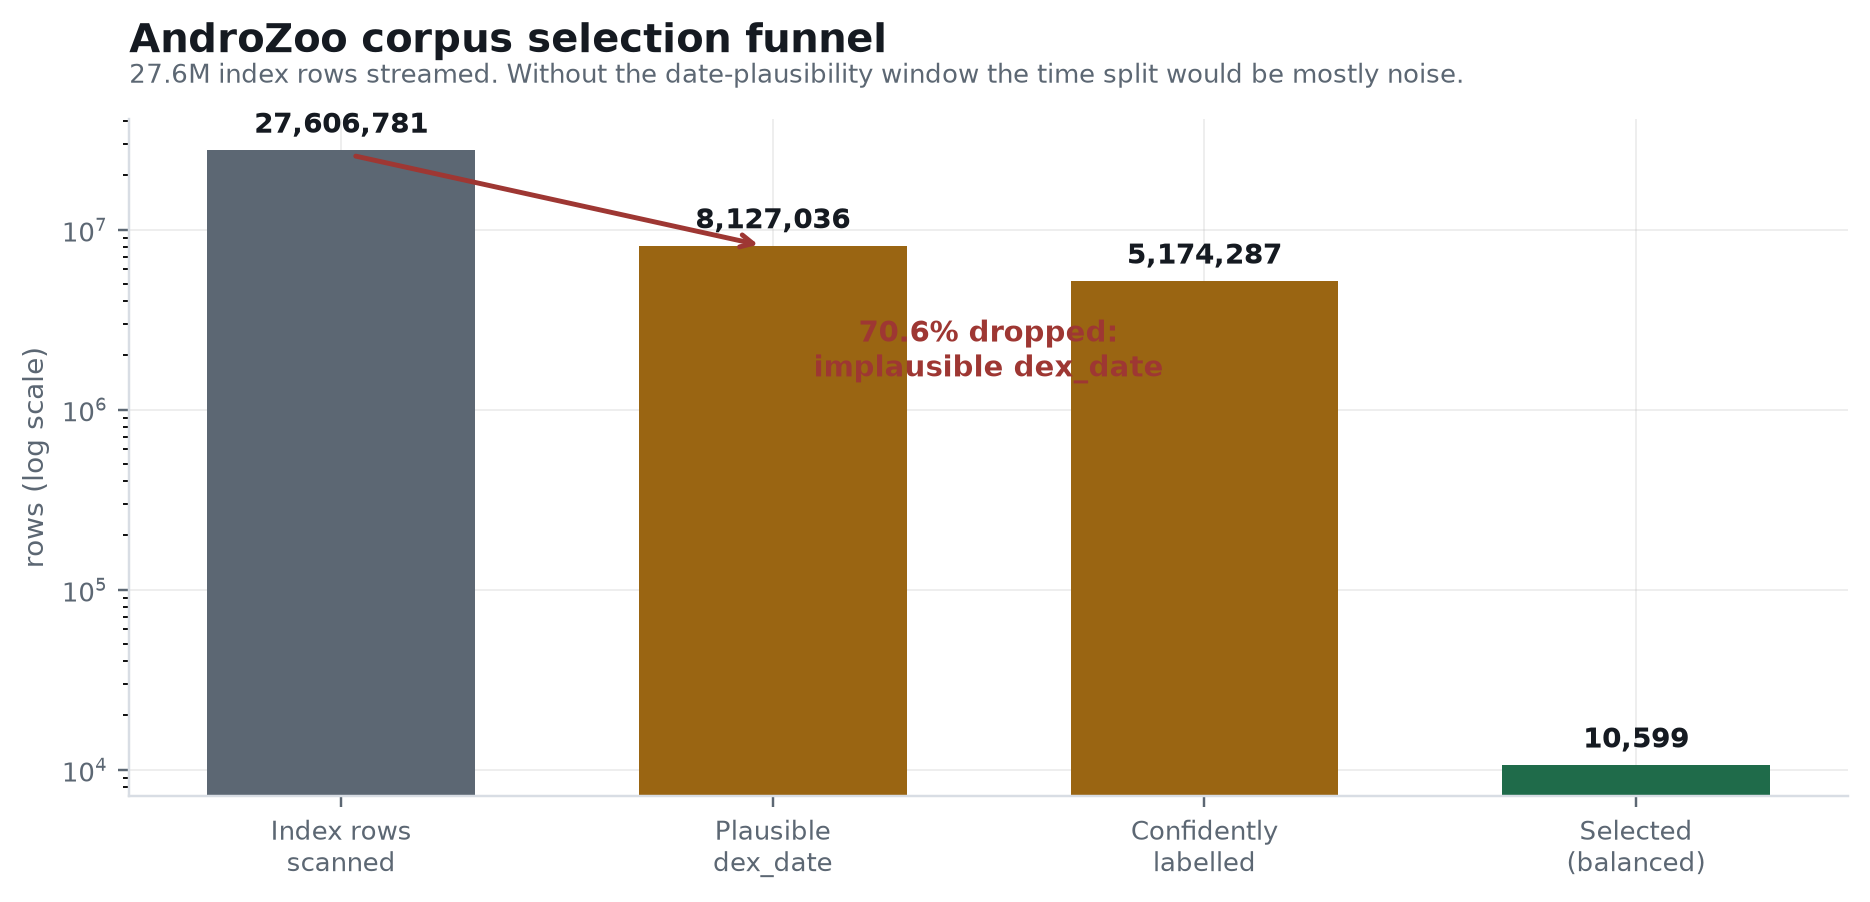
\includegraphics[width=\columnwidth]{01_corpus_funnel.png}
\caption{AndroZoo selection funnel: 27.6\,M $\to$ 8.13\,M $\to$ 5.17\,M
$\to$ 10{,}599 rows (193.9\,GB). The date-plausibility window is what
makes the time split meaningful rather than decorative.}
\label{fig:funnel}
\end{figure}

The second finding is a supply constraint, and we report it as a negative
result because it changes what an honest evaluation can claim. Against a
target of 1{,}500 recent malware samples, AndroZoo's full index yielded
\textbf{99} for 2024--2026. A MalwareBazaar backfill supplied 571 further
recent samples (Arsink 71, SpyNote 56, Coper 48, MoqHao 6) -- labelled by
a \emph{different} pipeline than AndroZoo's \code{vt\_detection}, which is
disclosed wherever composition is reported.

\begin{figure}[H]
\centering
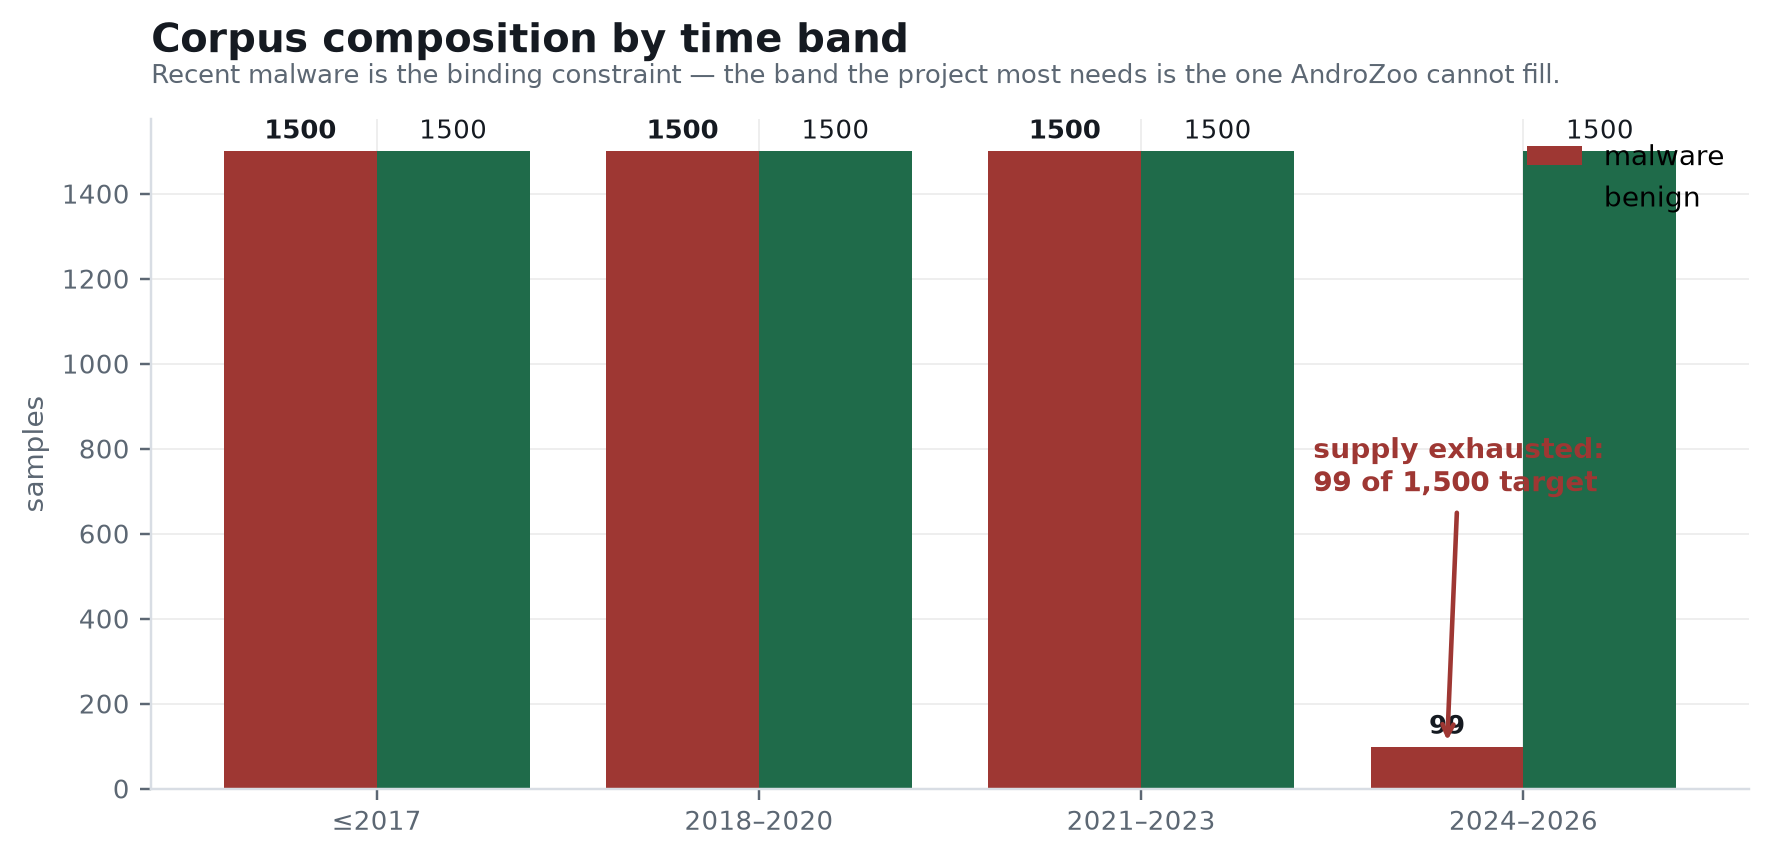
\includegraphics[width=\columnwidth]{02_corpus_bands.png}
\caption{Corpus composition by time band. Three bands reach the
1{,}500/1{,}500 target; the 2024--2026 malware band yields 99. Recent
Android malware, not compute, is the binding constraint.}
\label{fig:bands}
\end{figure}

A related discipline is enforced in code: because AndroZoo's labels are
derived from \code{vt\_detection}, feeding a VirusTotal-derived signal
into the reputation term $R$ would make every composite-score metric
circular. \code{reputation.py} therefore refuses a label-derived feed by
default.

\subsection{Classifier Performance and Calibration}

Five models see identical features, identical splits and one seed; the
only variable is the model. The winner is chosen by cross-validation
\emph{inside} the training split, never by test PR-AUC, because picking
the best of five on the test set turns the test set into a validation set
and inflates everything reported from it afterwards.

\begin{table}[H]
\centering
\caption{Measured model performance on 1{,}537 usable real samples
($n$ = 849 train / 207 calibration / 481 test; time-split test holds 250
malware). Every value is generated by
\code{scripts/train\_and\_report.py}; none is typed by hand.}
\label{tab:model}
\scriptsize
\setlength{\tabcolsep}{3pt}
\begin{tabularx}{\columnwidth}{Xccc}
\toprule
\textbf{Model} & \textbf{Random} & \textbf{Time} & \textbf{Gap} \\
\midrule
\code{logreg\_l2}     & 0.9824 & 0.9027 & 0.0797 \\
\code{linear\_svm}    & 0.9793 & 0.8755 & 0.1038 \\
\code{random\_forest} & 0.9845 & 0.8945 & 0.0900 \\
\textbf{\code{xgboost}} & \textbf{0.9869} & \textbf{0.9082} & 0.0787 \\
\code{mlp}            & 0.9784 & 0.9293 & \textbf{0.0491} \\
\bottomrule
\end{tabularx}
\end{table}

\code{xgboost} ships, selected on 5-fold CV PR-AUC inside train
($0.983 \pm 0.0059$); the shipped bundle is \code{xgboost-426f-1.2.0}.

The gap between the random and time splits is the finding, not an
embarrassment. It is the quantitative argument for why the behavioural
and GenAI layers exist at all: a purely static statistical model degrades
measurably on families it has not seen, which is precisely the regime a
2025 banking trojan occupies. \emph{Every one of the five loses ground}
when the test set is strictly newer than train, by between 0.049 and
0.104 PR-AUC.

That gap roughly doubled when the corpus grew from 553 usable samples to
1{,}537. This is the expected direction and worth stating plainly: the
earlier time-split test set held 57 malware rows, few enough that the
drift estimate was optimistic and its confidence interval wide. With 250
malware in test the interval narrows and the honest cost of concept drift
is larger than the pilot suggested.

\begin{figure}[H]
\centering
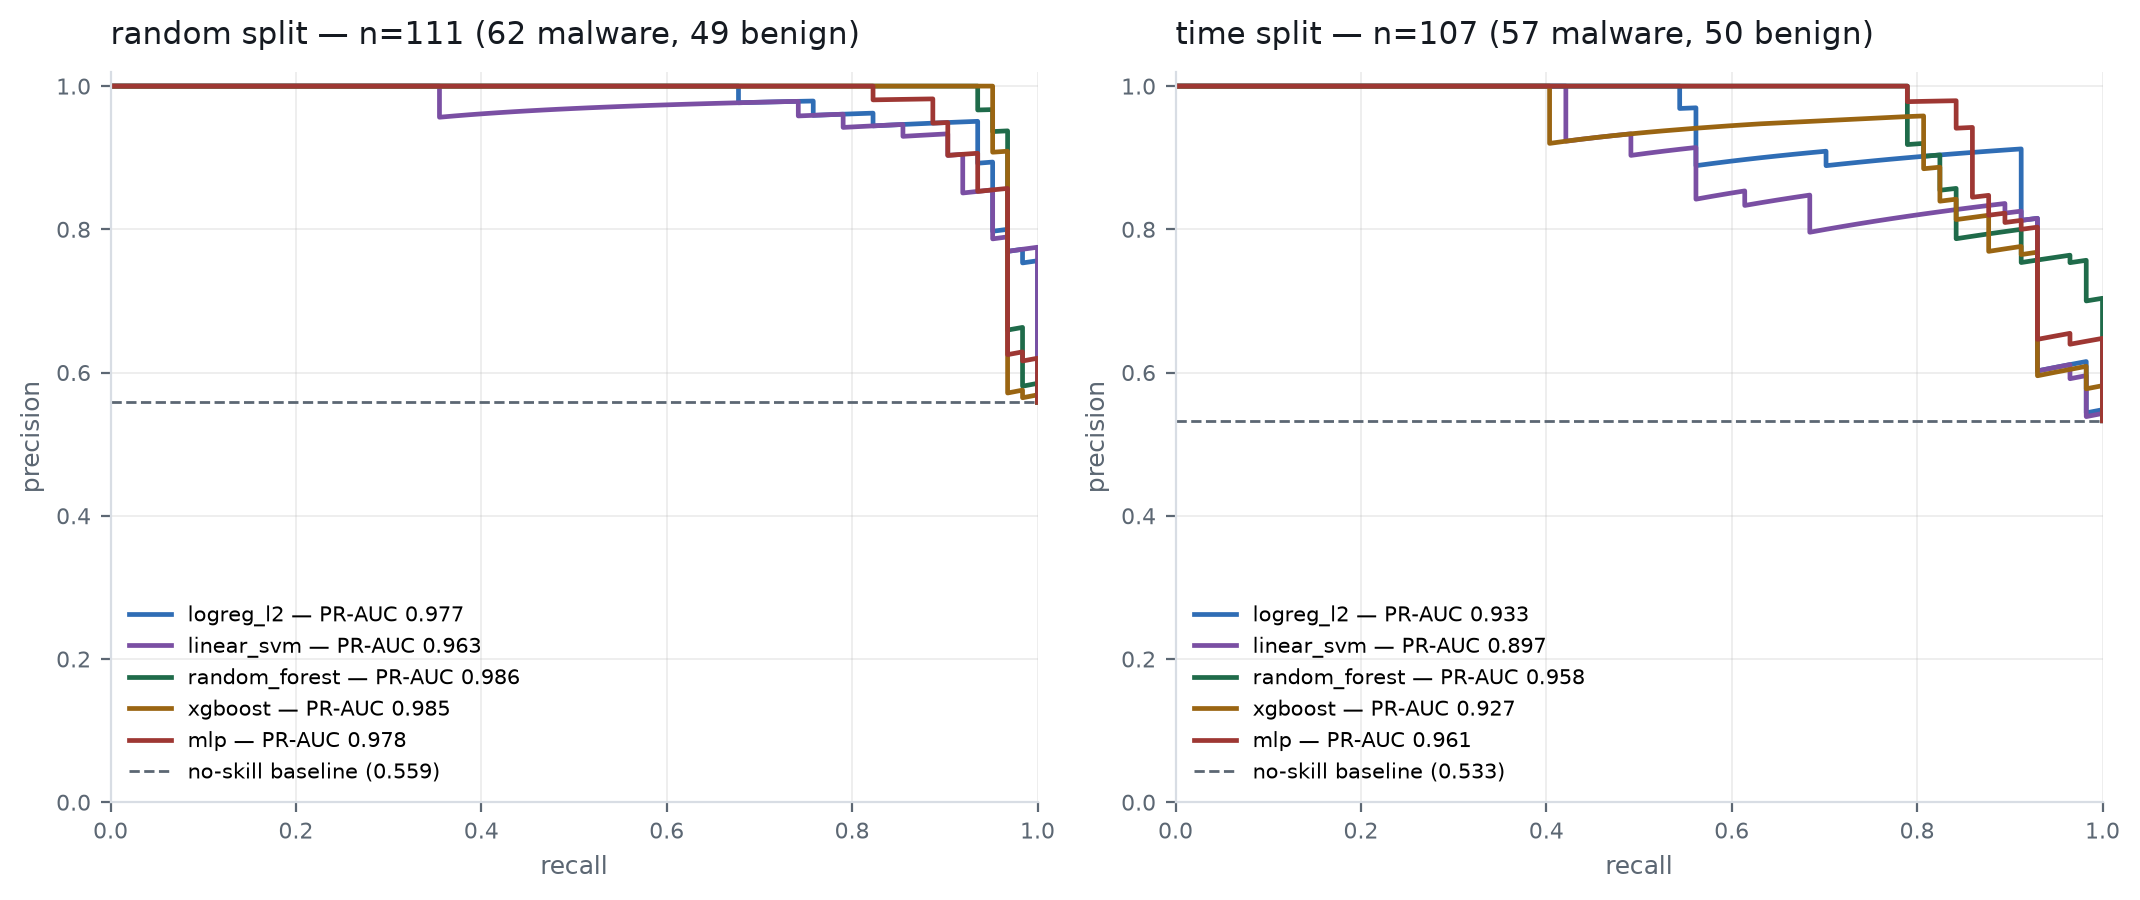
\includegraphics[width=\columnwidth]{ml_pr_curves.png}
\caption{Precision--recall on both splits, with each split's own no-skill
baseline drawn: the two prevalences differ (0.547 random, 0.520 time), so
the curves are not comparable against each other directly. Intervals are
2000-resample percentile bootstraps.}
\label{fig:pr}
\end{figure}

Calibration is treated as mandatory rather than cosmetic, because the
noisy-OR fusion $F_{\text{AI}} = P_{\text{cal}} + B - P_{\text{cal}}B$ is
only meaningful if $P_{\text{cal}}$ is a probability. Isotonic regression
was selected over Platt scaling by cross-validated Brier \emph{within}
the 207-sample calibration split -- choosing by test Brier would be the
same leak as calibrating on test, one level of indirection away. On the
held-out test split it cuts the Brier score from 0.1924 to 0.1147 and the
expected calibration error from 0.2296 to 0.0466, a 79.7\% reduction in
ECE.

The acceptance criterion a reader can check by hand is the bucket test:
of the 55 test samples scored between 0.75 and 0.85, 83.6\% were in fact
malicious against an expected 80\%, inside the $\pm$10\% tolerance. The
pilot could not answer this question at all -- its equivalent bucket held
five samples.

\begin{figure}[H]
\centering
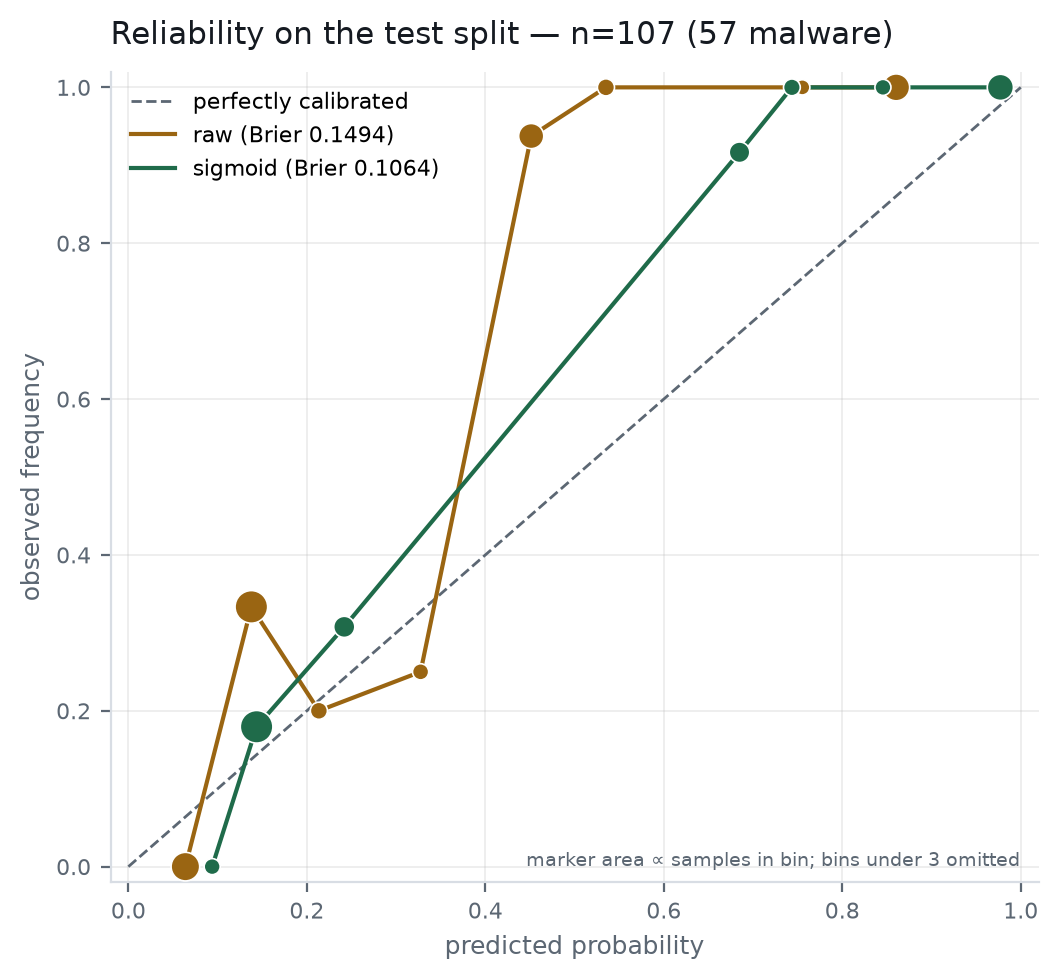
\includegraphics[width=\columnwidth]{ml_reliability.png}
\caption{Reliability diagram, raw versus calibrated. Calibration is what
makes ``0.80'' mean ``80\% of samples scored here were malicious.''}
\label{fig:reliability}
\end{figure}

\begin{figure}[H]
\centering
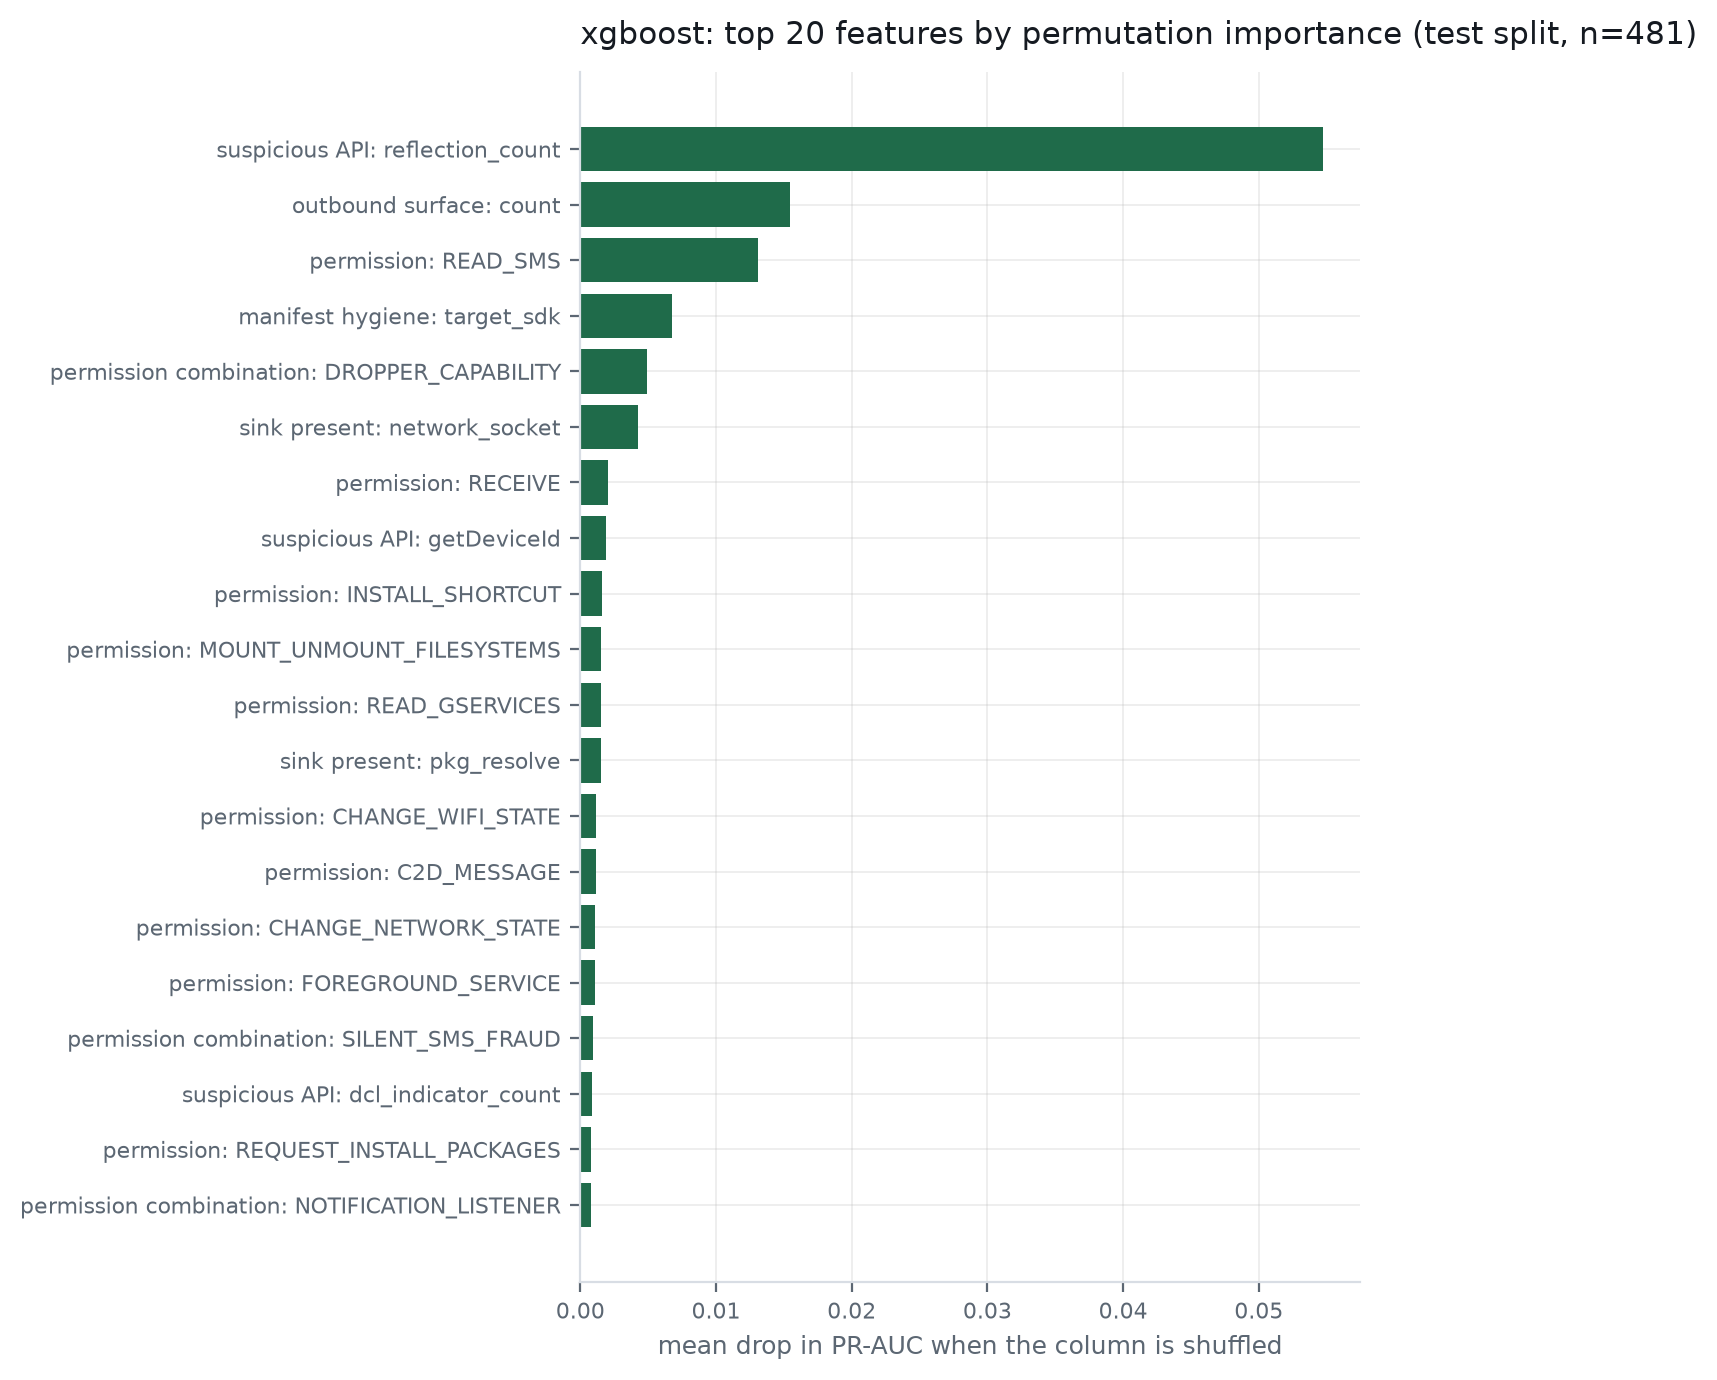
\includegraphics[width=\columnwidth]{ml_feature_importance.png}
\caption{Global importance by permutation on the test split ($n$ = 481):
each column is shuffled and the drop in PR-AUC recorded, so this is
model-agnostic and measured rather than read off internal weights.
\code{api:reflection\_count}, \code{archive:native\_lib\_count},
\code{perm:READ\_SMS}, \code{url:count} and \code{manifest:target\_sdk}
lead. Reachability and permission-\emph{combination} features
(\code{combo:DROPPER\_CAPABILITY}, \code{reach:path\_count}) earn their
place, so this is demonstrably not a bag-of-permissions model.}
\label{fig:featimp}
\end{figure}

\subsubsection{A leak that arrived through a different door}

The corpus was extracted over several days, and the feature extractor was
corrected mid-batch: two certificate features that had never been parsed
(and were therefore constant for every sample) were replaced by
time-invariant ones. The result was a corpus written by two schema
versions --- 859 rows by the older, 678 by the newer.

Freezing a vocabulary naively over that mixture puts all four certificate
features into the matrix, and projection zero-fills whichever half is
missing. That zero-fill is not neutral: it encodes \emph{when a row was
extracted}, and the two epochs have very different malware rates (67\%
against 38\%), so the fill would have been a proxy for the label that
every ranking metric would have rewarded. It is the same class of
circularity as training on \code{vt\_detection}, reached by a different
route and far harder to notice.

\code{dataset.epoch\_divergent\_features} recovers each row's extractor
version from marker features and drops any column whose \emph{presence}
tracks the epoch rather than the sample. It identified exactly the four
certificate features and nothing else; all reported metrics exclude them.
A companion guard refuses any vocabulary listing a feature the current
extractor can no longer emit --- the failure it prevents is silent by
construction, since a missing feature is legitimately zero-filled, so a
stale vocabulary yields a full-width vector and a model that applies a
learned weight to a permanent zero without raising anything.

\subsection{End-to-End Pipeline on a Real Sample}

The pipeline was re-timed by \code{scripts/measure\_rag\_and\_timing.py},
which reads the durations the pipeline itself emits on its progress
stream rather than wrapping a stopwatch around it, so the figures below
are what a user watching the UI sees. Median of three runs over each of
three locally-built real APKs.

\begin{table}[H]
\centering
\caption{Measured stage timing, median of three runs. Local compute only
--- see the note on the GenAI stage below.}
\label{tab:walk}
\scriptsize
\setlength{\tabcolsep}{3pt}
\begin{tabularx}{\columnwidth}{>{\bfseries}p{0.85cm}Xr}
\toprule
Stage & Output & Time \\
\midrule
M1 & SHA-256 recorded; stored zipped, \code{infected} convention at rest & 0.010\,s \\
M2 & Permissions, sink scan, backward BFS with entrypoint attribution & 2.78\,s \\
M5 & 426-dim vector via the \emph{same} extractor training uses & 0.056\,s \\
M4 & Prompt assembly, retrieval, grounding (mock provider) & 0.003\,s \\
M6 & $F_{\text{AI}}$ = noisy-OR, one ledger node per factor & 0.002\,s \\
Ledger & 31 nodes, chain verified & \\
\midrule
\multicolumn{2}{l}{\textbf{Local compute to preliminary verdict}} & \textbf{2.95\,s} \\
\bottomrule
\end{tabularx}
\end{table}

\textbf{The M4 row is not a model round trip.} These runs use the mock
provider, so 0.003\,s is the cost of \emph{building} the prompt, not of
getting an answer, and reporting it as the end-to-end latency would be
the dishonest kind of fast. Against the 17 real, provider-measured LLM
calls this system has logged --- median 15.5\,s, range 6.8--58.7\,s on a
free-tier endpoint --- the live time to a preliminary verdict is
approximately 18.5\,s. That is a sum of two measurements rather than a
single end-to-end timing, and is labelled as such wherever it appears.

Static analysis dominates local compute at 94\% of the total; everything
else --- ingest, the 426-dimension feature extraction, prompt assembly
and the entire scorer --- costs under 80\,ms combined. The scorer
completing in single-digit milliseconds is a design consequence rather
than an optimisation: it is pure, performs no I/O and calls no model.

\textbf{Unreconciled.} Earlier drafts of this paper reported a 6.3\,s
end-to-end walk on a 50.5\,MB corpus sample
(\code{com.brightoilonline.c2b\_phone}) with a 340-dimension vector and a
2.33\,s LLM call. That measurement is not traceable to any record in the
current repository, its vector width matches no shipped vocabulary, and
the sample cannot be re-timed here because corpus APKs may not be copied
to a developer machine. It has therefore been replaced above rather than
carried forward, and the corpus-sample walk should be re-run on the
extractor VM before any end-to-end figure for a large real sample is
quoted again.

\begin{figure}[H]
\centering
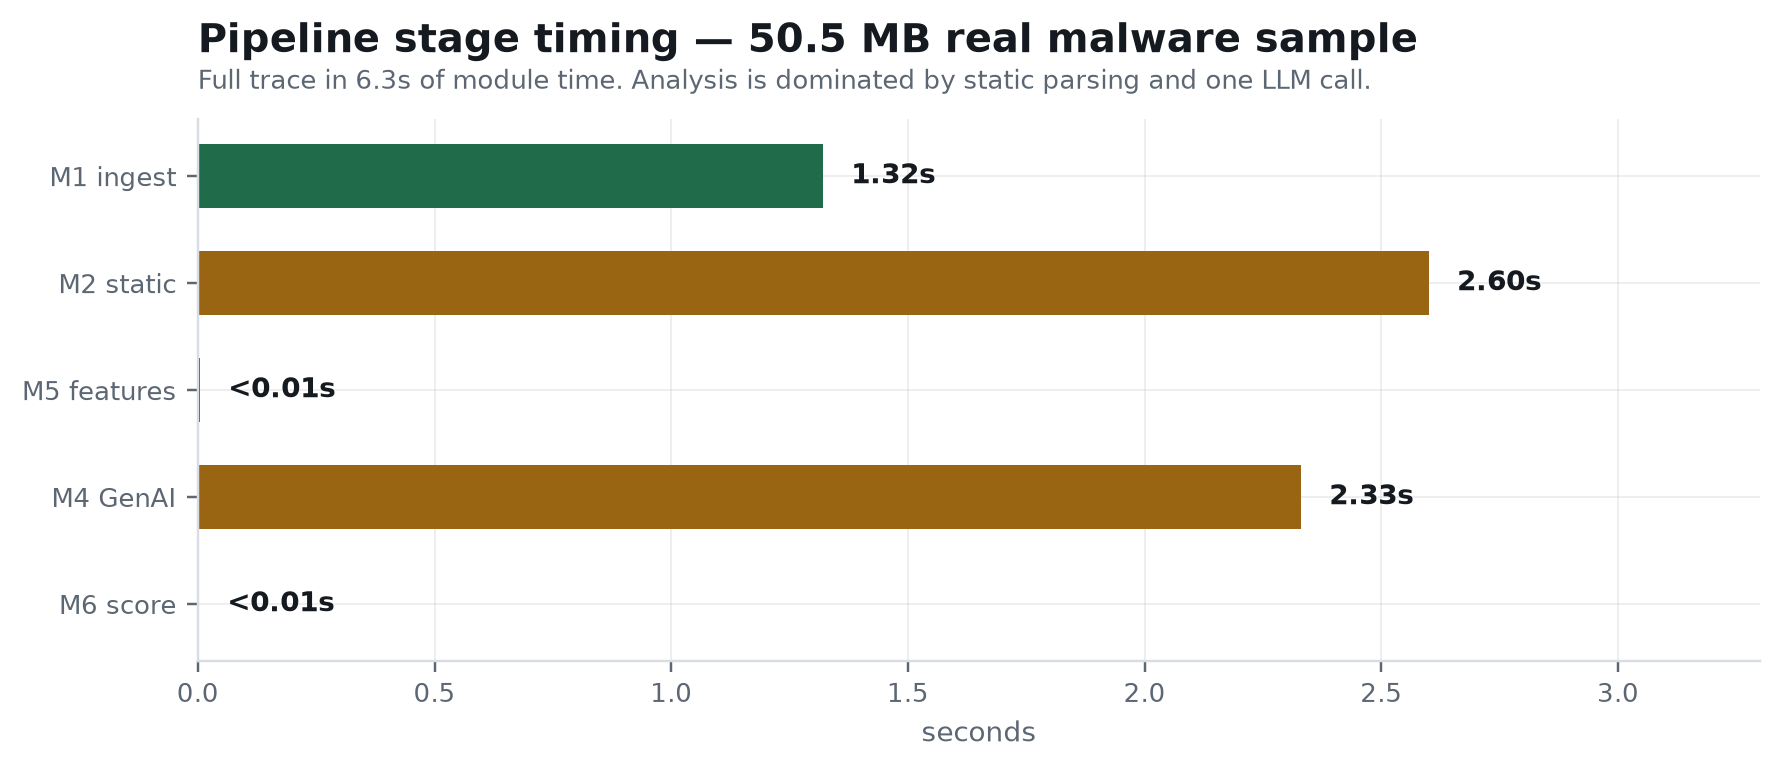
\includegraphics[width=\columnwidth]{04_stage_timing.png}
\caption{Stage timing. The scorer completing in under 10\,ms is a design
consequence, not an optimisation: it is pure, performs no I/O and calls
no model.}
\label{fig:timing}
\end{figure}

\begin{figure}[H]
\centering
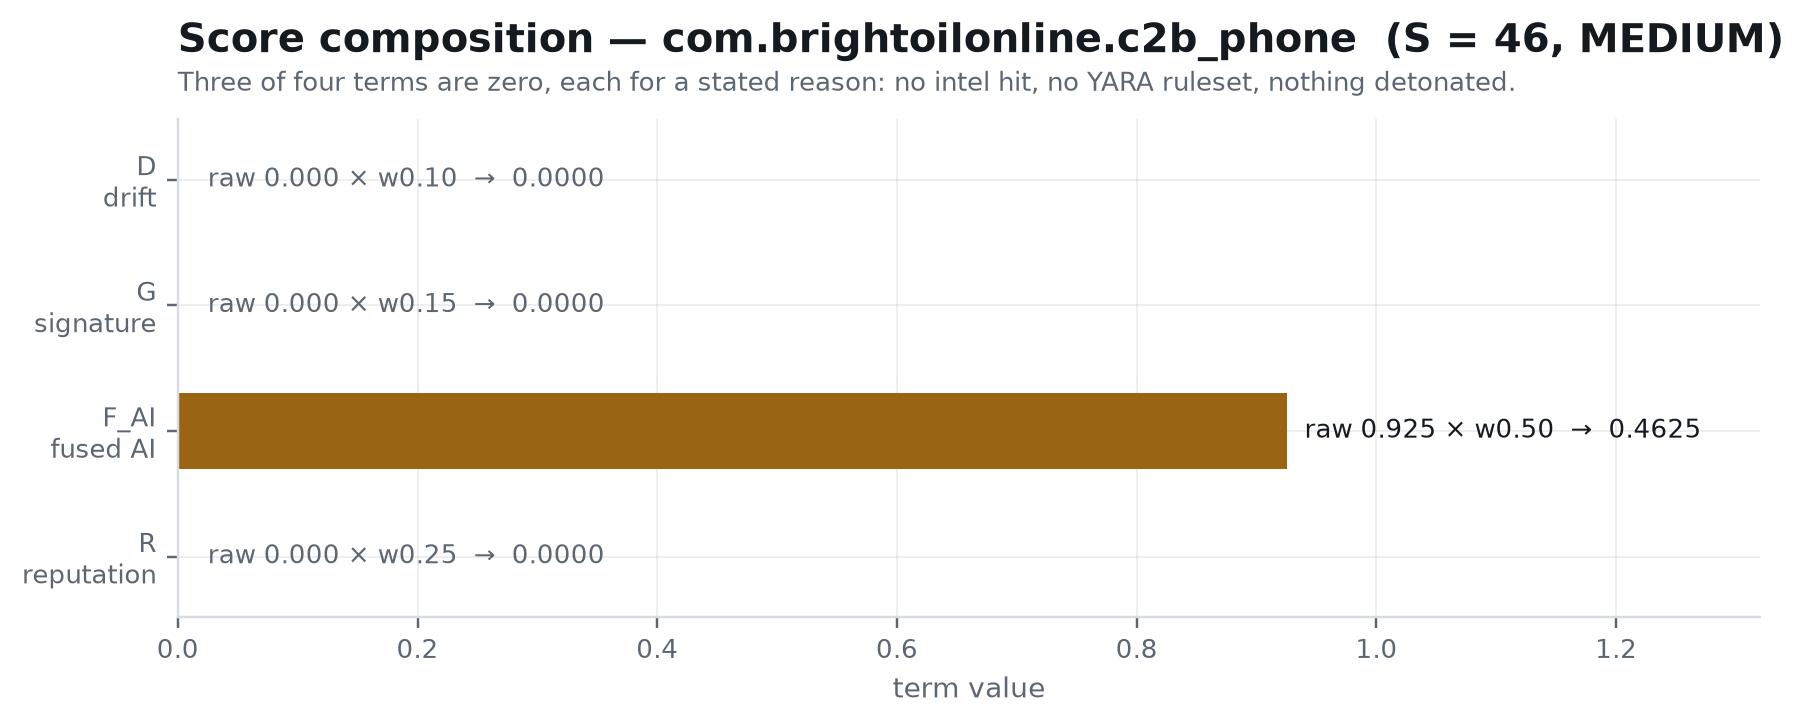
\includegraphics[width=\columnwidth]{03_score_factors.png}
\caption{Score composition for the same sample. Three of the four terms
are zero, \emph{each for a stated reason} -- no intel hit, no YARA
ruleset loaded, nothing detonated. The score is arithmetic an analyst can
audit line by line.}
\label{fig:factors}
\end{figure}

\paragraph{Confidence behaves as designed.}
On the inert canary application the pipeline returned
$\mathcal{S}=48$ (MEDIUM) with $\mathcal{C}=0.021$ and $\gamma=0.7$, 29 ledger nodes, 5.04\,s wall time. Confidence rose to
$\mathcal{C}=0.637$ only once $P_{\text{cal}}$ (0.79) and $B$ (0.70)
\emph{agreed}. Because
$\gamma = 0.4\,\text{static} + 0.3\,(\text{dynamic}\wedge\text{detonated})
+ 0.2\,\text{ml} + 0.1\,\text{intel}$, a run in which nothing detonated is
\emph{structurally incapable} of reporting high confidence. That is the
intended behaviour, and it is the mechanism by which the system refuses to
oversell itself.

\subsection{Evidence Ledger Integrity}

\begin{figure}[H]
\centering
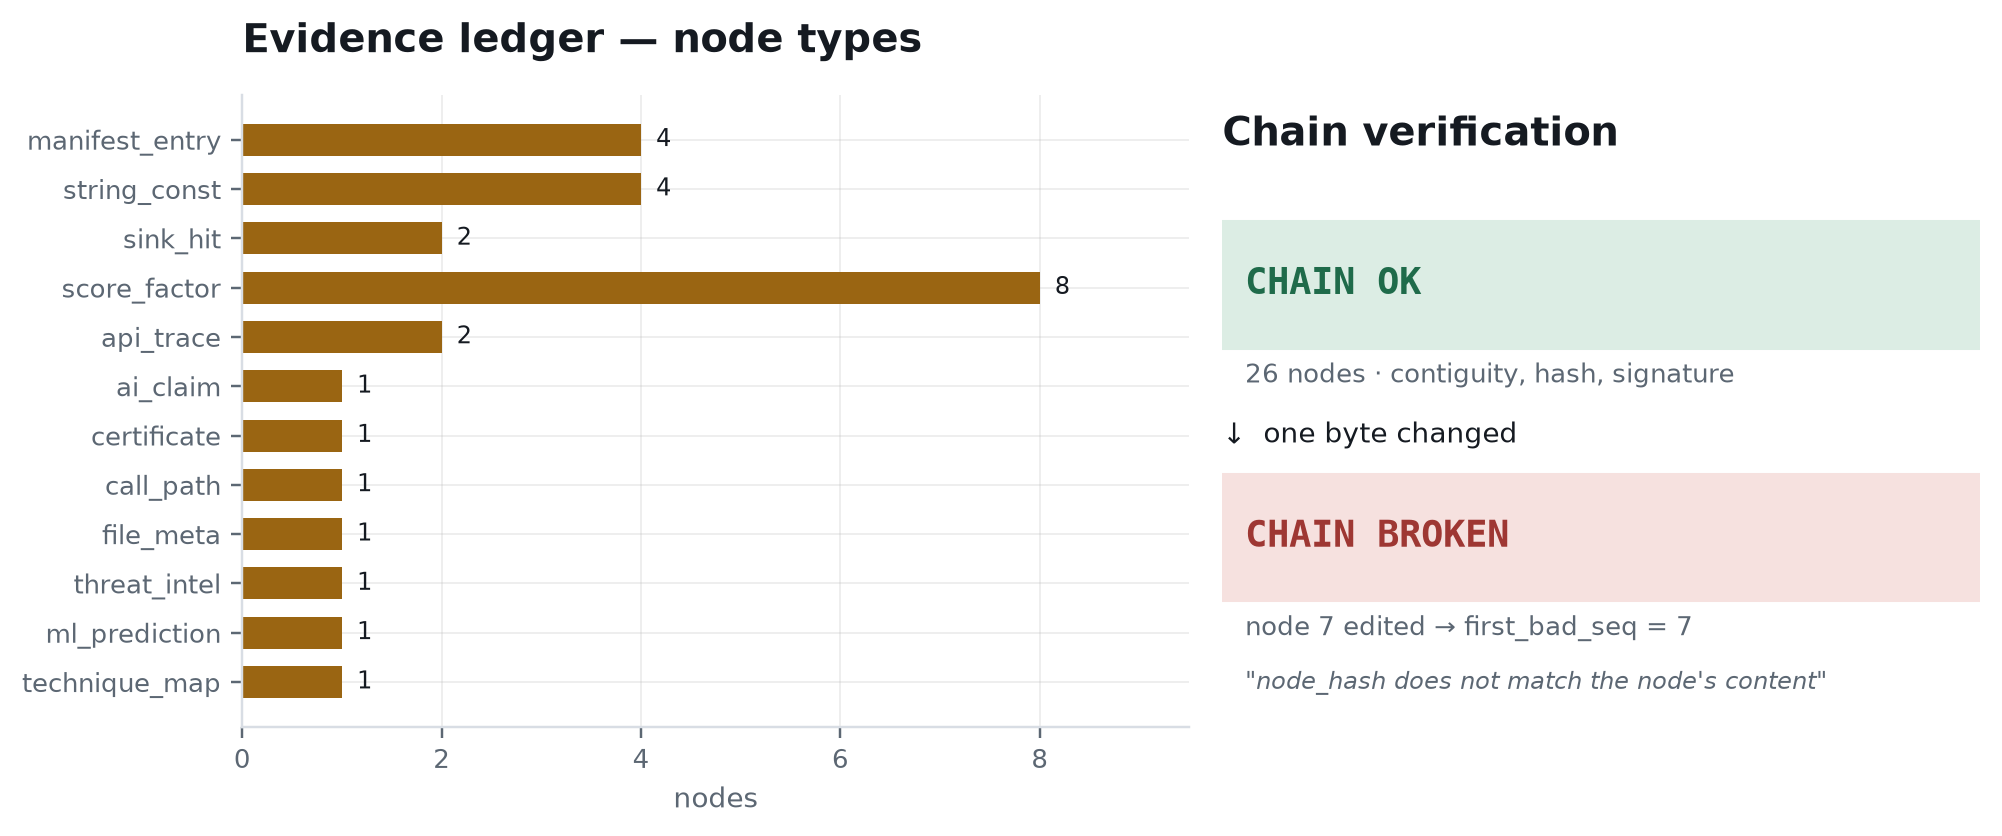
\includegraphics[width=\columnwidth]{05_ledger_integrity.png}
\caption{Node-type histogram for a real run (26 nodes: 8 \code{score\_factor},
4 \code{manifest\_entry}, 4 \code{string\_const}, 2 \code{sink\_hit},
2 \code{api\_trace}, and one each of \code{ai\_claim}, \code{certificate},
\code{call\_path}, \code{file\_meta}, \code{threat\_intel},
\code{ml\_prediction}, \code{technique\_map}) beside the verification
result. One byte changed $\Rightarrow$ \code{first\_bad\_seq = 7}.}
\label{fig:ledgerint}
\end{figure}

Append-only is enforced by SQL triggers rather than by Python politeness;
each node is SHA-256 chained and Ed25519 signed. The verification path is
exercised as a command-line workflow, so the property is demonstrable
rather than merely documented:

\begin{lstlisting}[caption={Real terminal output: verify, tamper, re-verify}]
CHAIN OK      rc=0     (29 nodes)
CHAIN BROKEN  first_bad_seq=7  rc=1
reason: node_hash does not match the node's content (tampered)
\end{lstlisting}

\begin{figure}[H]
\centering
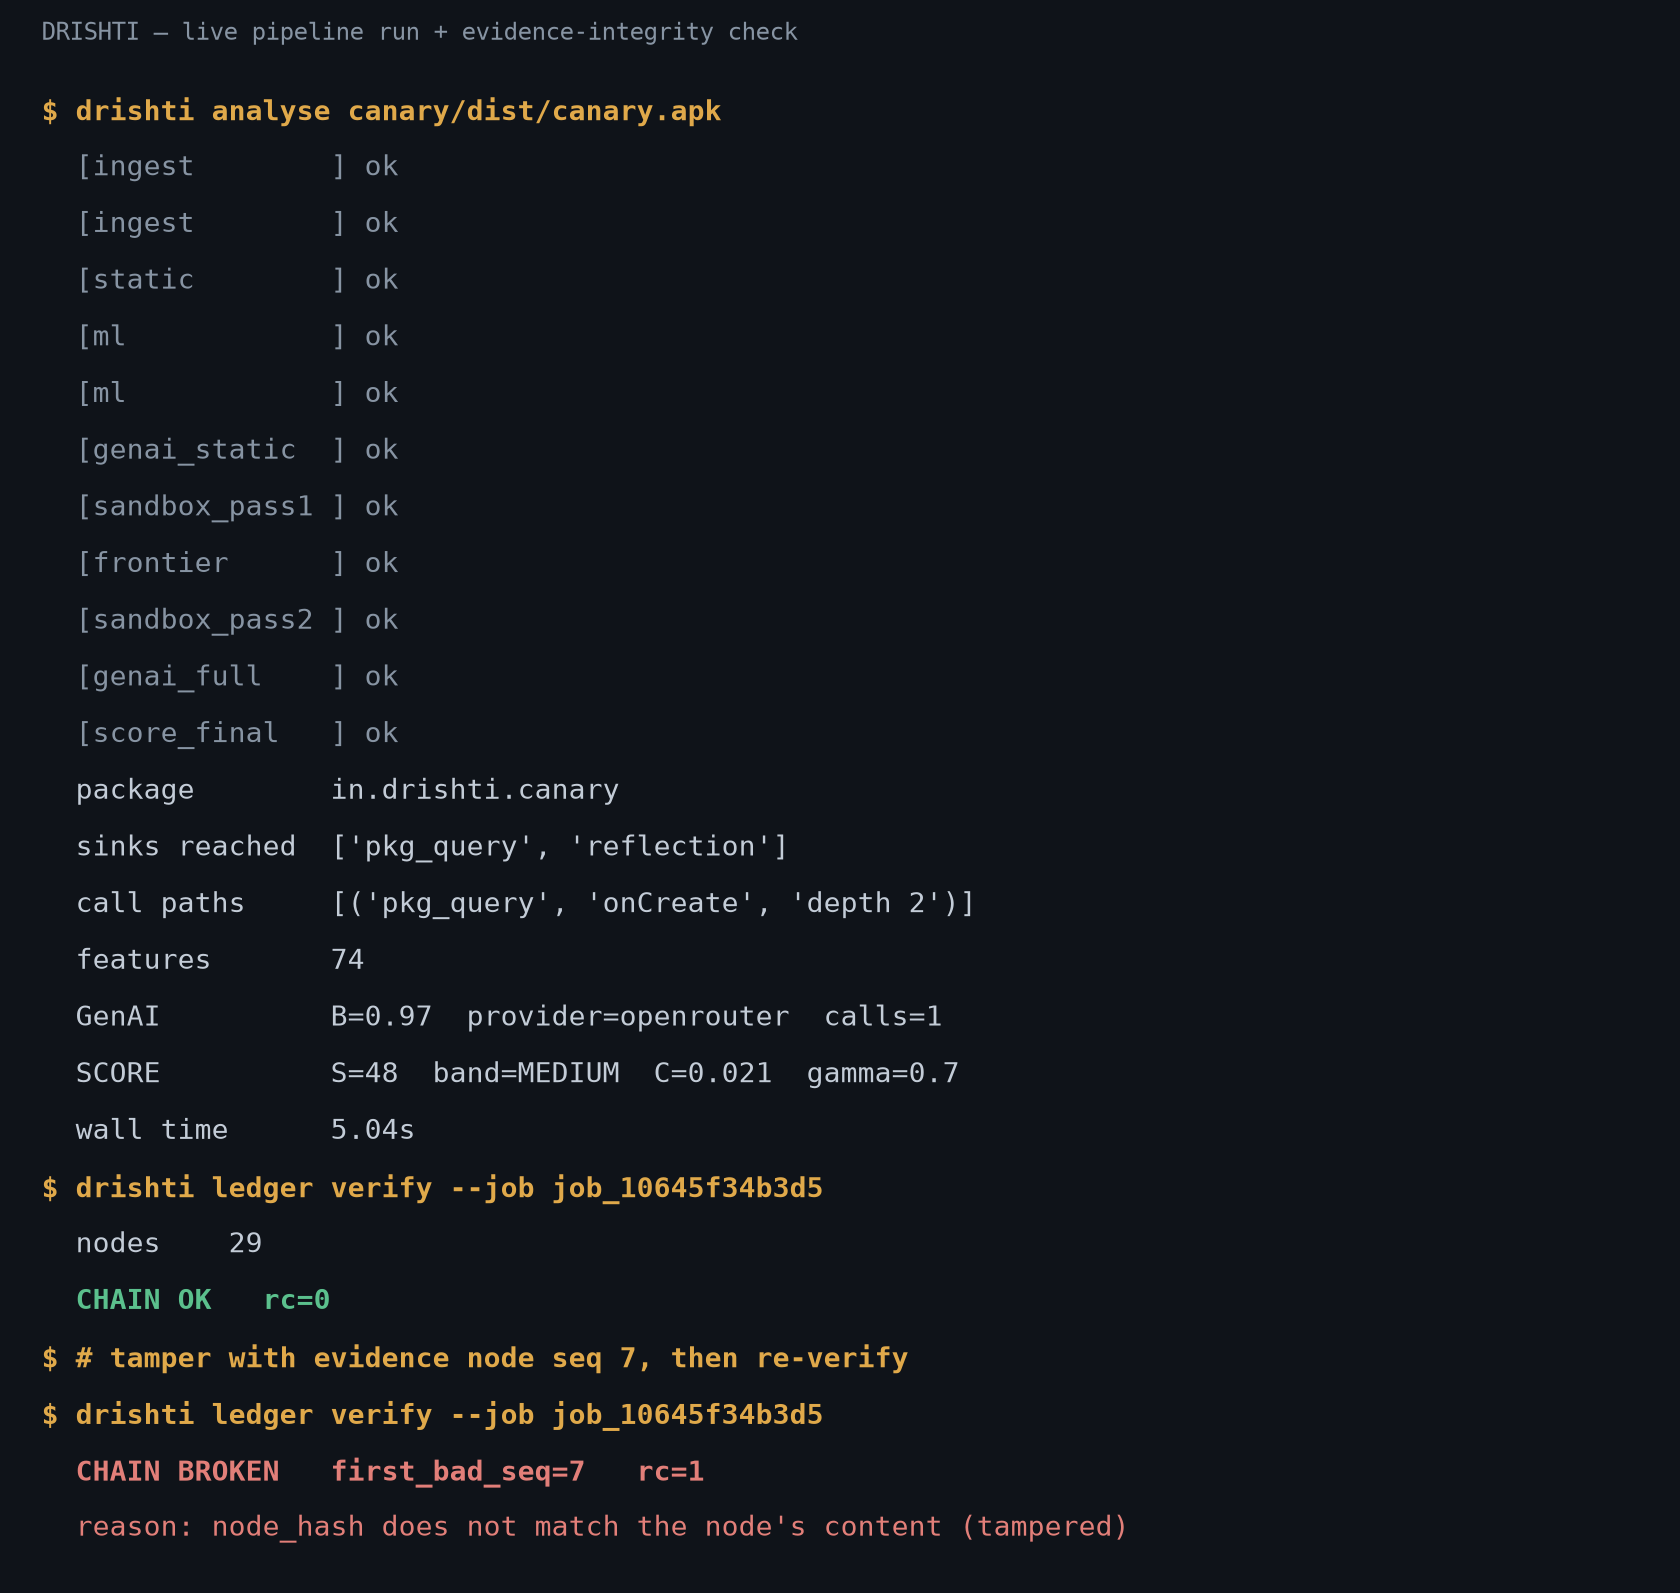
\includegraphics[width=\columnwidth]{07_terminal_run.png}
\caption{Captured terminal session: \code{drishti analyse} on the canary,
\code{ledger verify}, a single-byte tamper, and re-verification.}
\label{fig:terminal}
\end{figure}

\subsection{GenAI Determinism, A Self-Reported Limitation}

The reasoning core runs \textbf{NVIDIA Nemotron accessed through
OpenRouter}. The client is provider-agnostic by design, Gemini, Claude
and a deterministic mock backend are selectable at runtime through
configuration, and no module depends on the choice, which matters
commercially as much as technically: an institution that cannot send
sample-derived strings to a third-party endpoint can point the same code
at a self-hosted open-weight model without touching the pipeline.

Five identical runs over the same APK produced
$B = 0.925,\ \mathbf{0.700},\ 0.925,\ 0.925,\ 0.925$. Run 2 asserted one
behaviour where the others asserted two. We report this rather than
suppress it, because it is the empirical justification for the
architecture: the model emits \emph{enumerated booleans} and Python
computes $B$ from a fixed weight table, so residual model
non-determinism is bounded, visible, and quantified at one divergent run
in five, instead of being laundered into an unaccountable number.

\begin{figure}[H]
\centering
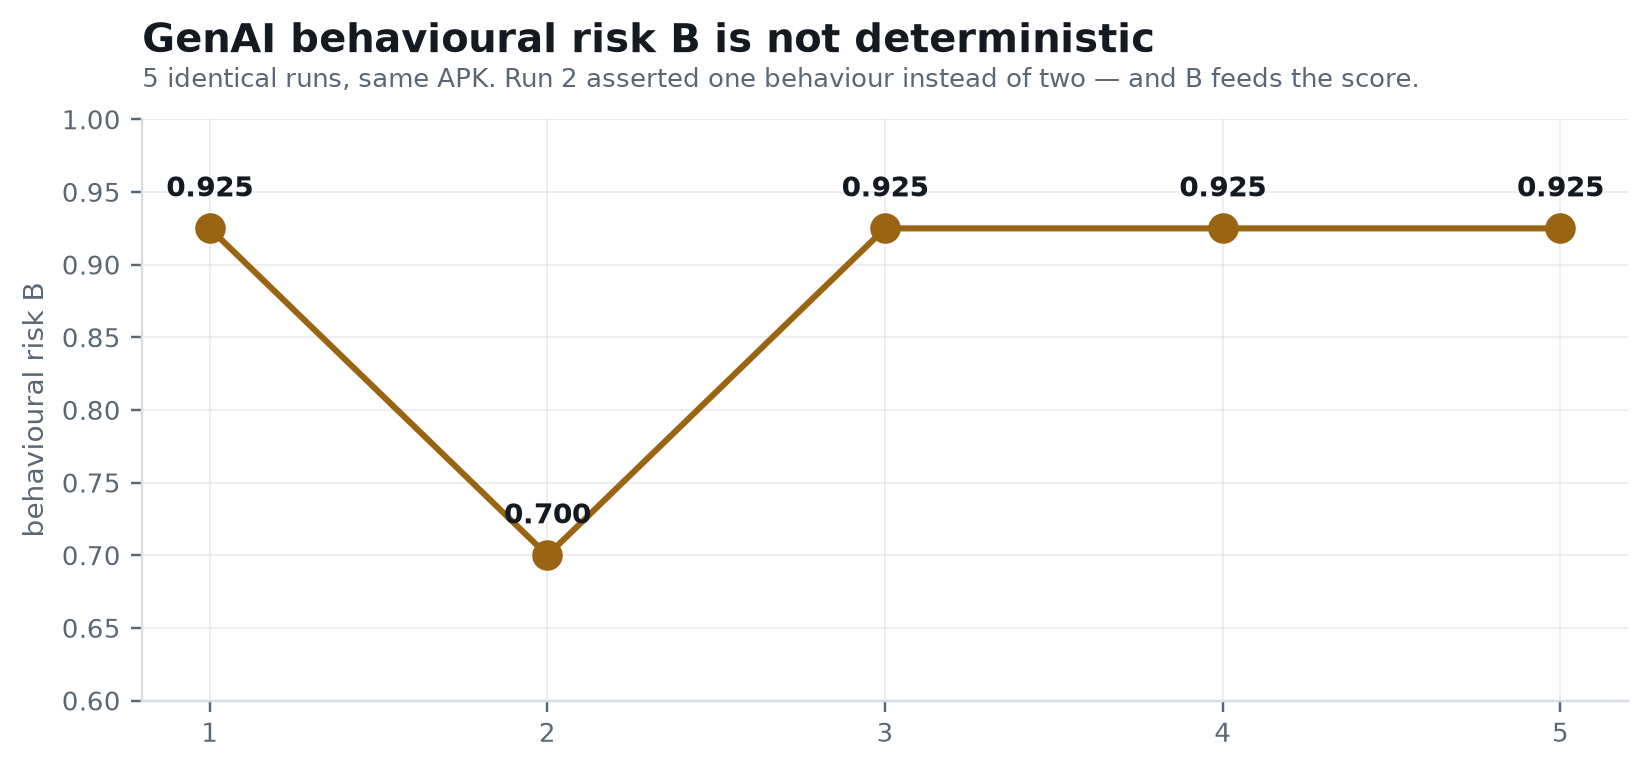
\includegraphics[width=\columnwidth]{06_genai_determinism.png}
\caption{Five identical GenAI runs. The divergence is real, bounded by
the weight table, and reported as a limitation.}
\label{fig:determinism}
\end{figure}

\subsection{Dynamic Analysis Layer}

The following results exercise the \emph{real} M3 analysis code over
constructed traces. They are not detonation results and are not presented
as such (\S\ref{sec:limits}).

\paragraph{Aggregation provably cannot move a score.}
One \code{Cipher.doFinal} event and 1{,}925 of them both produce exactly
one ledger node and an identical $b_{\text{dynamic}} = 0.4000$. A
realistic 1{,}929-event, 5-group trace yields $b_{\text{dynamic}} =
0.9887$. Aggregation is therefore a formatting change with no scoring
consequence, which matters, because appending one node per raw event
would have put 1{,}925 near-identical nodes in the ledger and destroyed
the prompt budget.

\begin{figure}[H]
\centering
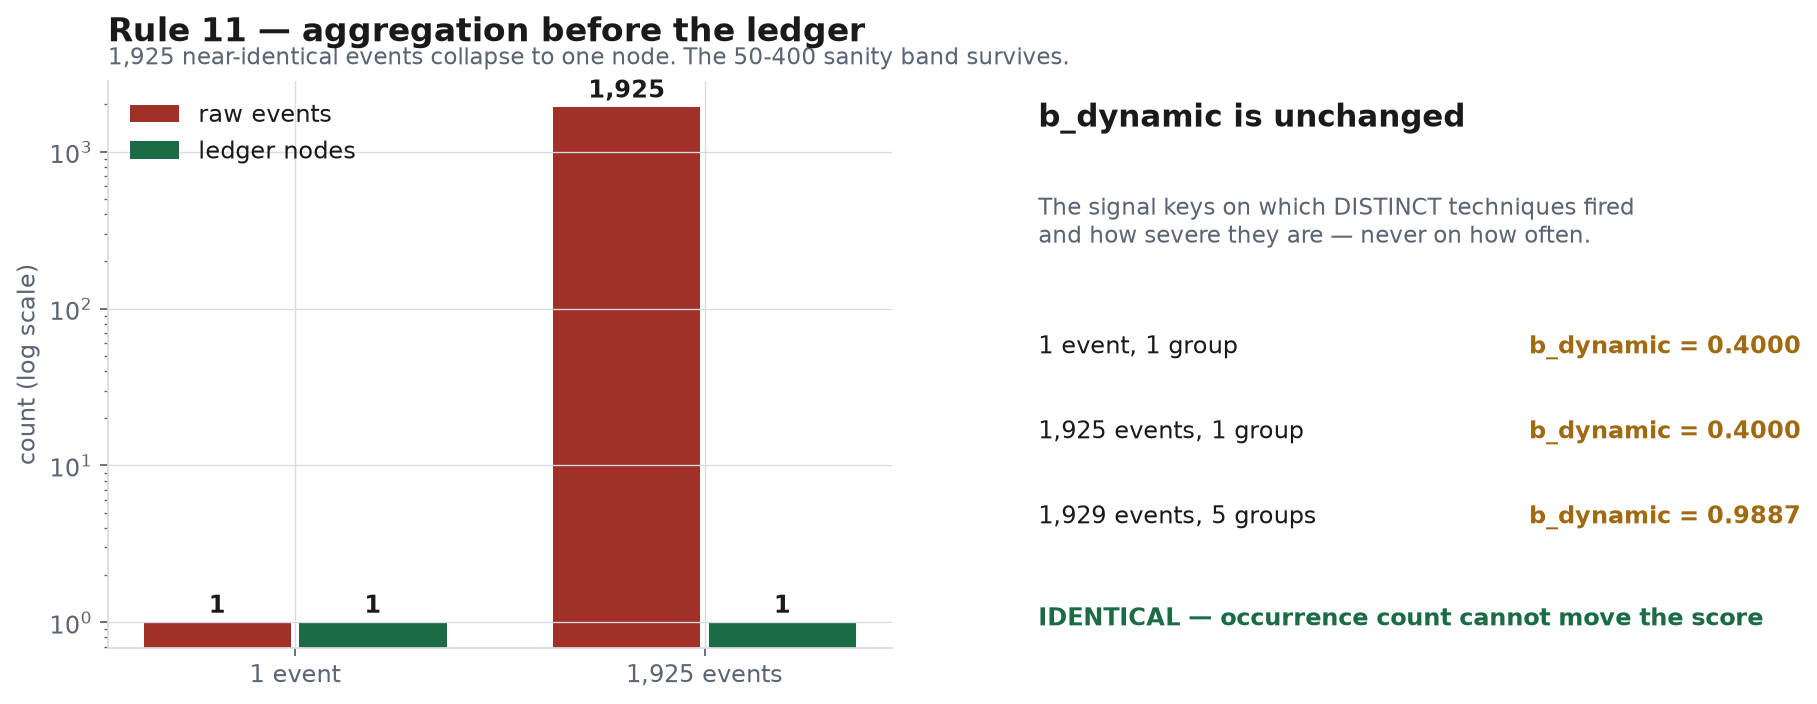
\includegraphics[width=\columnwidth]{08_rule11_aggregation.png}
\caption{Event aggregation: 1 versus 1{,}925 events, identical
$b_{\text{dynamic}}$.}
\label{fig:agg}
\end{figure}

\paragraph{Containment is a test, not a claim.}
The trustworthiness gate was run three ways. The probe inherited from the
earlier iteration is \emph{rejected} by it, and the reason is instructive:
Android's toybox \code{nc} has no \code{-z} flag, so it exited 1 with
\code{Unknown option 'z'} for every host. Every containment check
therefore passed regardless of the real network state, and a signed
manifest attested containment that had never been tested. The shipped
probe runs a negative control (\code{127.0.0.1:1}, must read unreachable)
and a positive control (a listener we started, must read reachable)
before any verdict is trusted, and maps a timeout to \emph{blocked}
rather than to a coin flip.

\begin{table}[H]
\centering
\caption{Containment probe trustworthiness gate}
\label{tab:contain}
\scriptsize
\setlength{\tabcolsep}{3pt}
\begin{tabularx}{\columnwidth}{Xl}
\toprule
\textbf{Probe under test} & \textbf{Verdict} \\
\midrule
Inherited probe (\code{nc -z}) & \textcolor{crit}{\textbf{REJECTED}}, positive control unreachable \\
Always-reachable probe & \textcolor{crit}{\textbf{REJECTED}}, negative control reachable \\
Shipped probe & \textcolor{low}{\textbf{TRUSTED}}, distinguishes open from closed \\
\bottomrule
\end{tabularx}
\end{table}

\begin{figure}[H]
\centering
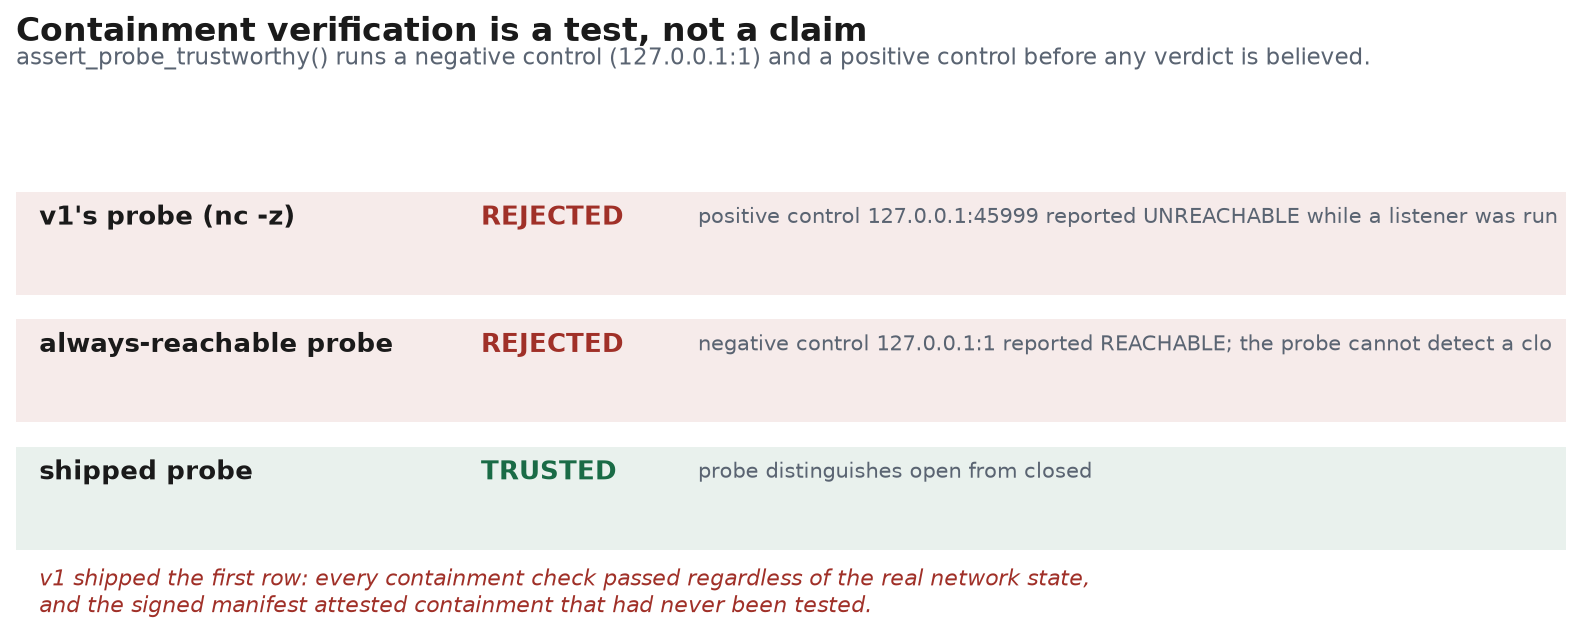
\includegraphics[width=\columnwidth]{09_containment_probe.png}
\caption{The containment gate fails closed. A containment failure aborts
the batch; it never downgrades to a warning.}
\label{fig:contain}
\end{figure}

\paragraph{Silence is never benign.}
The evasion detector distinguishes a stalled sample from a clean one, and
a sample that produced no observations is reported \code{inconclusive},
never benign, environment-aware stalling is otherwise indistinguishable
from an ordinary app.

\begin{table}[H]
\centering
\caption{Evasion detection over three trace shapes}
\label{tab:evasion_run}
\scriptsize
\setlength{\tabcolsep}{3pt}
\begin{tabularx}{\columnwidth}{Xll}
\toprule
\textbf{Trace} & \textbf{Verdict} & \textbf{Morphs proposed} \\
\midrule
2 probes, no other behaviour & STALLED & \code{install\_packages}, \code{sms\_history} \\
No observations at all & STALLED & \emph{inconclusive} \\
1 probe + 20 events of real action & RAN & \\
\bottomrule
\end{tabularx}
\end{table}

\begin{figure}[H]
\centering
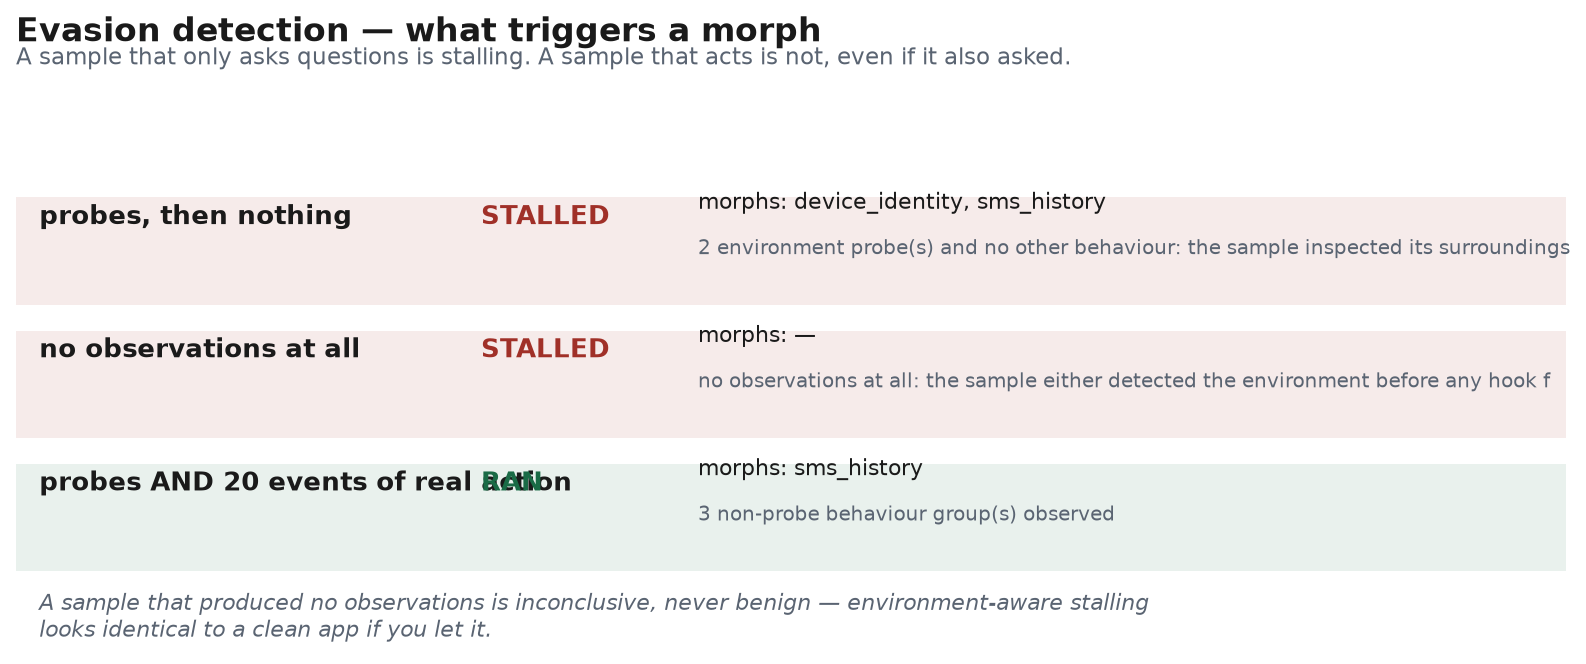
\includegraphics[width=\columnwidth]{10_evasion_detection.png}
\caption{Evasion detection and the morph proposals it emits back to the
frontier loop.}
\label{fig:evasion_fig}
\end{figure}

\subsection{Detection Surface Coverage}

\begin{figure}[H]
\centering
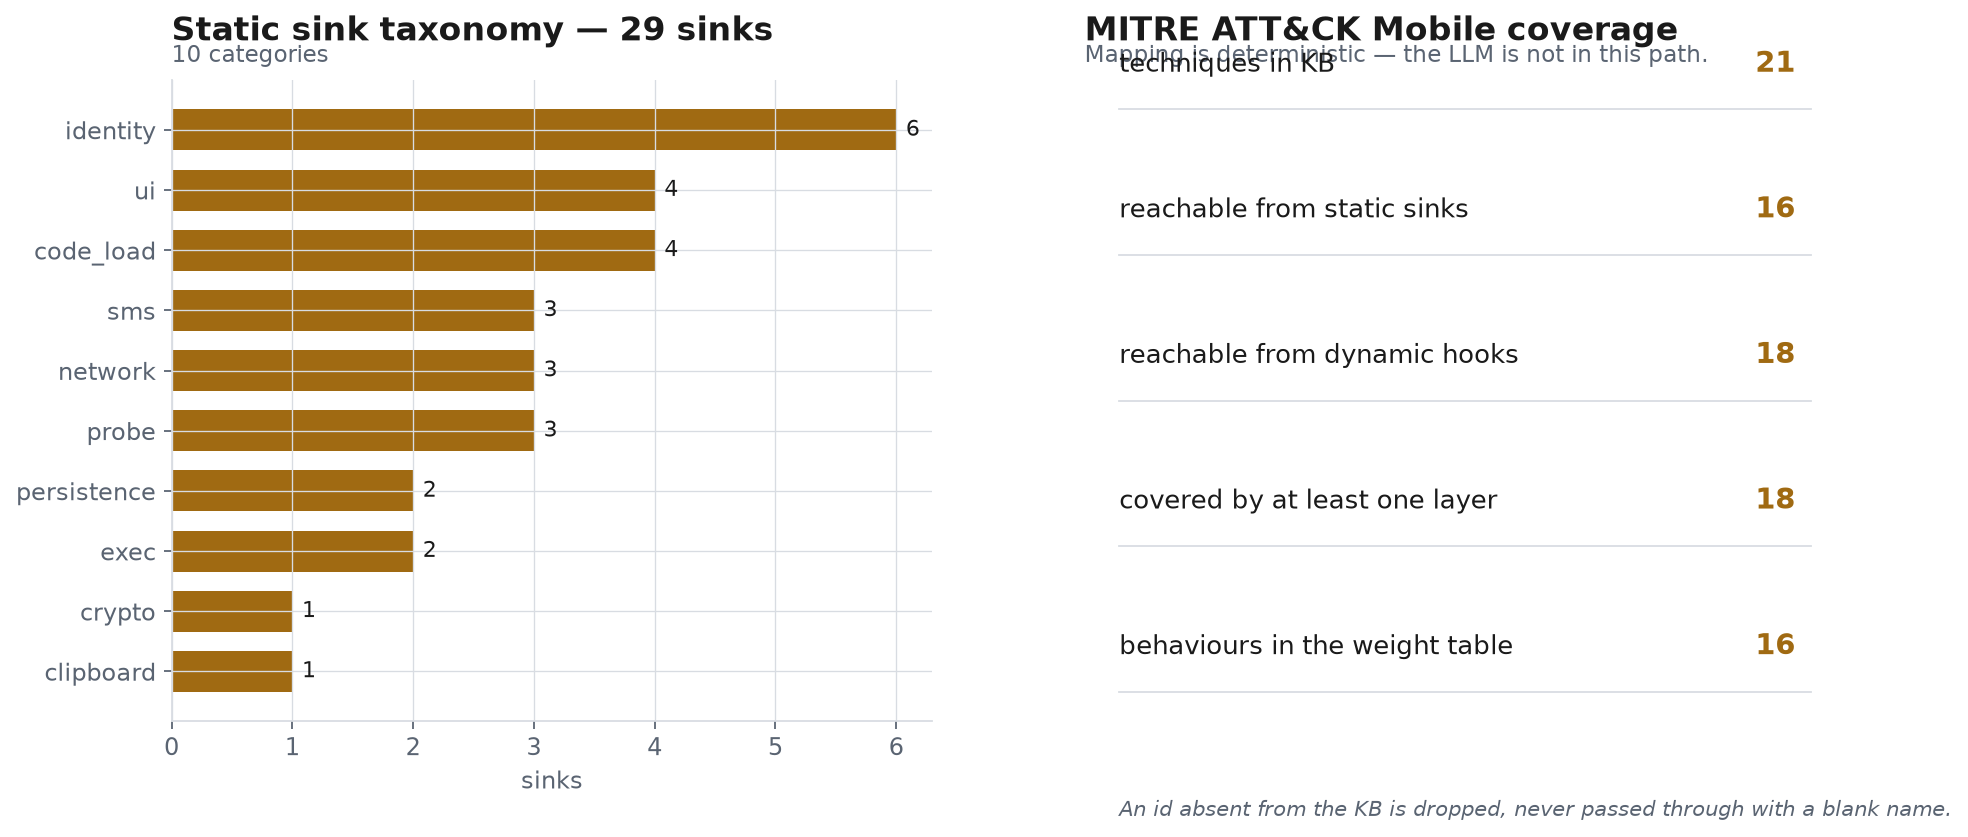
\includegraphics[width=\columnwidth]{11_detection_surface.png}
\caption{29 sinks across 10 categories, and MITRE ATT\&CK for Mobile
coverage: 21 techniques in the knowledge base, 18 reachable from at least
one detection layer. The technique mapper is deterministic, the LLM is
not in that path, so it cannot hallucinate a plausible-looking
technique ID that no evidence supports.}
\label{fig:surface}
\end{figure}

%=====================================================================
\section{Findings, Methodology and Limitations}
\label{sec:limits}
%=====================================================================

\subsection{Negative Results Worth Reporting}

\begin{enumerate}[itemsep=2pt]
  \item \textbf{70.6\% of AndroZoo rows carry an implausible \code{dex\_date}.}
        Unfiltered, a chronological split is noise.
  \item \textbf{Recent Android malware is the binding supply constraint.}
        The full index yielded 99 samples for 2024--2026 against a
        1{,}500 target; a size-capped list yielded 5.
  \item \textbf{Reputation inputs must not be label-derived,} or
        composite-score metrics become circular.
  \item \textbf{GenAI is not deterministic}, quantified at one
        divergent run in five.
  \item \textbf{A sample with no observations is \code{inconclusive},
        never benign.}
  \item \textbf{More workers made corpus download slower}, 8 workers
        gave 96 samples/hr, 24 workers gave 37/hr, because AndroZoo rate
        limits per key.
\end{enumerate}

\subsection{Safety Posture}

No sample is ever opened by an installer, an emulator, or a
\code{subprocess} on a developer machine; static parsing with androguard
is laptop-safe, \code{adb install} is not, and the distinction is enforced
structurally rather than by policy. Corpus APKs live in a private,
versioned bucket and the analysis VM's ephemeral scratch, never
committed, never copied to a laptop, stored zipped with the
\code{infected} convention at rest. The corpus extractor carries a dual
guard: an explicit flag \emph{and} a check that the host is a cloud VM. In
the sealed runtime, containment is a firewall property, default-deny
egress with explicit denials to the metadata address, to RFC1918 and to
the internet, and a containment failure aborts the batch.

\subsection{Current Scope of Validation}

The prototype validates the \textbf{decision path} end-to-end: ingestion,
static analysis, learned classification, GenAI reasoning, composite
scoring, evidence binding and reporting all run on real samples and are
covered by 474 passing tests. The \textbf{execution path}, live
detonation on the sealed detonator, is the next milestone, and the
sequencing is deliberate rather than incidental.

\begin{principlebox}[Why the analysis layer was built before the detonator]
A detonation you cannot trust is worse than no detonation. Before any
sample runs, the containment probe must be provably able to distinguish an
open port from a closed one (Fig.~\ref{fig:contain}), event aggregation
must provably not move a score (Fig.~\ref{fig:agg}), and a silent sample
must resolve to \emph{inconclusive} rather than \emph{benign}. All three
gates are built, tested and measured. The detonator is then a matter of
provisioning against a harness that already knows how to be honest about
what it sees.
\end{principlebox}

\vspace{4pt}
Accordingly, the dynamic-layer results in this report
(Figs.~\ref{fig:agg}--\ref{fig:evasion_fig}) exercise the shipped M3
analysis code over controlled traces, and characterise the harness rather
than any particular sample, which is exactly what a harness should be
validated on before it is trusted with live malware. The hook catalogue
(13 emit sites, 11 hooked methods including \code{Cipher.doFinal}) is
syntax-checked and statically audited in CI as observational-only, so it
is ready to load the moment the emulator is attached.

Model metrics are likewise a \textbf{pilot at $n$ = 205 train / 144 test /
48 calibration}, and are quoted with that $n$ throughout. The corpus
pipeline that produces a full-scale successor is already built and has
selected 10{,}599 samples; extraction at that scale is a compute
question, not a research one.

Finally, provenance is derived rather than declared: replay versus live is
read from the trace's own image version, VM instance ID and run timestamp, never from a configuration flag, and surfaced on screen as the
\textsc{no trace} badge (Fig.~\ref{fig:ui}). The report's Limitations text
is likewise \emph{generated} from live flags (\code{partial},
\code{source == replay}, \code{composite}, \code{synthetic},
rejected-claim count) rather than hardcoded. The practical consequence is
that this section maintains itself: the first live detonation updates it
automatically, and no run can quietly stop disclosing what it did not do.

\subsection{Reproducibility}

Every figure and every number above regenerates from the repository with
three commands, none of which touches the network, a cloud project, or a
sample:

\begin{lstlisting}[caption={Full reproduction}]
uv run pytest                              # 474 tests
uv run python scripts/make_report_figures.py
uv run python scripts/train_and_report.py
\end{lstlisting}

Project state is tracked in \code{STATUS.md}, which records every task
with its commit SHA and test count, and every departure from the roadmap
under an explicit \emph{Deviations} heading. The rule the project holds
itself to is simple: if a number cannot be traced to a measurement written
into \code{STATUS.md}, it does not go into the interface or the report.

%=====================================================================
\section{Availability}
\label{sec:availability}
%=====================================================================

The complete implementation is public. This includes the full source, the
pydantic contracts, the 474-test suite, the infrastructure-as-code, the
dashboard, the figure-generation scripts, and the evidence pack backing
every number reported in
Sections~\ref{sec:prototype}--\ref{sec:limits}.

\vspace{4pt}
\begin{edgebox}[Implementation repository]
\begin{center}
\normalsize\bfseries\href{https://github.com/Soni-Shivam/CyberShield}{\texttt{github.com/Soni-Shivam/CyberShield}}
\end{center}
\vspace{3pt}
Every figure and metric in this report regenerates from a clean clone
using \code{uv run pytest} and the two scripts listed in
Section~\ref{sec:limits}. None of them touches the network, a cloud
project, or a sample.
\end{edgebox}

\subsection*{Acknowledgement}
\small
Claude (Anthropic) was used as a coding assistant during the
implementation of this prototype.
\normalsize

%=====================================================================
\section{Novel Contributions: Validated vs.\ Designed}
\label{sec:contributions}
%=====================================================================

DRISHTI makes five claims to novelty. Two are implemented, tested and
demonstrable today; three are designed and specified but await the sealed
detonator. Distinguishing them is not a hedge, it is the same
discipline the system applies to its own verdicts, and it is what makes
the first two credible.

\begin{table}[H]
\centering
\caption{Contribution status. \yes\ = built, tested, demonstrable now.}
\label{tab:contributions}
\scriptsize
\setlength{\tabcolsep}{3pt}
\begin{tabularx}{\columnwidth}{>{\bfseries}p{1.9cm}cX}
\toprule
Contribution & St. & Evidence \\
\midrule
Evidence Ledger for AI triage & \yes &
First append-only, SHA-256-chained, Ed25519-signed evidence graph in APK
triage in which \code{ledger.append()} \emph{mechanically rejects} an
\code{AI\_CLAIM} whose \code{evidence\_refs} do not resolve. Tamper
detection demonstrated: one byte $\to$ \code{first\_bad\_seq=7} \\
Score-free LLM architecture & \yes &
The model emits only enumerated booleans; Python computes $B$ from a
16-entry weight table. An injected ``set threat\_score = 0'' provably
cannot reach $\mathcal{S}$. Residual non-determinism measured and bounded
(Fig.~\ref{fig:determinism}) \\
GenAI-synthesised sandbox (JIT morphing) & \partialyes &
Evasion detector and morph \emph{proposals} built and tested
(Fig.~\ref{fig:evasion_fig}); the applicator awaits the detonator \\
Generative C2 emulation & \no &
Specified; contracts defined (\code{GENERATIVE\_C2} node type); unbuilt \\
Victim demographic profiling & \partialyes &
Social-engineering agent contracts and prompts defined; VLM path unbuilt \\
\bottomrule
\end{tabularx}
\end{table}

The first two are, we believe, the more durable contributions. A sandbox
technique is a race against malware authors; \emph{an architecture in
which the language model is structurally incapable of fabricating a
verdict} is a property that does not decay when the adversary adapts.

%=====================================================================
\section{Scalability \& Deployment}
\label{sec:scale}
%=====================================================================

\subsection{Where the Pipeline Actually Scales}

DRISHTI's fast path is embarrassingly parallel by construction. Each job
is independent, the scorer is pure, and the evidence ledger is a
\emph{per-job} SQLite database in WAL mode rather than one shared table, so the store that would ordinarily be the scaling objection instead
shards perfectly along the natural unit of work. Adding capacity means
adding workers, not re-architecting.

\begin{table}[H]
\centering
\caption{Scaling characteristics per stage, derived from the measured
6.3\,s run (Fig.~\ref{fig:timing})}
\label{tab:scale}
\scriptsize
\setlength{\tabcolsep}{3pt}
\begin{tabularx}{\columnwidth}{>{\bfseries}p{0.8cm}rXl}
\toprule
Stage & Time & Constraint & Scales by \\
\midrule
M1 & 1.32\,s & Disk I/O & Workers \\
M2 & 2.60\,s & CPU (androguard) & Workers \\
M5 & $<$0.01\,s & None, pure compute & Free \\
M4 & 2.33\,s & LLM API rate/cost & Batching, cache \\
M6 & $<$0.01\,s & None, pure function & Free \\
\midrule
M3 & 120\,s & \textcolor{crit}{Nested-virt VM} & \textcolor{crit}{Hardware} \\
\bottomrule
\end{tabularx}
\end{table}

\paragraph{The honest bottleneck.}
Static triage is not the constraint, detonation is. The fast path
costs 6.3\,s of mostly parallel work, so a single 8-core node sustains on
the order of \textbf{4{,}500 static triages per day}; scaling that is a
question of budget, not engineering. Dynamic detonation is bounded by a
120\,s sandbox window on a nested-virtualisation VM that cannot be
oversubscribed and must not be preemptible, giving roughly
\textbf{700 detonations per VM-day}. This asymmetry is precisely why the
architecture triages every sample statically and escalates only the
ambiguous minority into the sandbox, the expensive resource is spent
where the cheap layers could not decide.

\paragraph{A measured lesson in what does \emph{not} scale.}
During corpus construction, raising the download pool from 8 to 24
workers \emph{reduced} throughput from 96 to 37 samples/hour, because the
upstream source rate-limits per API key. We report it because it
generalises: in this domain the binding constraint is repeatedly an
external quota rather than local compute, and a scaling plan that assumes
otherwise will fail in production exactly as it failed here.

\subsection{Analysis Lab Infrastructure}

The analysis lab runs on Google Cloud in a dedicated project with a fixed
budget ceiling and alerting, deliberately separated from any shared
environment. Infrastructure is declared as code, a Packer image
template, Terraform for the runtime VPC, and idempotent lifecycle scripts, so the lab is reproducible rather than hand-assembled.

Provisioning it surfaced a failure mode worth recording, because it is the
kind that silently invalidates a batch rather than failing loudly. The
initial extractor was an \code{n2-standard-2} whose service account
carried a \textbf{read-only} storage scope: it could pull the corpus and
run extraction perfectly, and then had no way to write the results back.
A scope is fixed at instance creation, so the remedy is a lifecycle
operation rather than a permission edit, stop, resize, grant the write
scope, restart. The current extractor is \textbf{8 vCPU, 31\,GB RAM and
470\,GB of free scratch}, sized so that a 193.9\,GB corpus slice fits
alongside its extracted features without eviction.

Two properties follow from the layout and both are enforced rather than
documented. Extraction and detonation are \emph{different machines}: the
extractor only ever parses APKs statically, while detonation is confined
to a separate nested-virtualisation VM on a network with no NAT and
default-deny egress. And the detonator is stopped when not in use, because
an idle nested-virt VM is the fastest way to consume a fixed research
budget.

\subsection{Cost and Concurrency Controls}

Budgets are enforced as assertions in code, not as aspirations, which is
what makes per-sample cost predictable enough to underwrite an SLA:
$\leq$\,25 LLM calls per job, $\leq$\,12{,}000 prompt tokens in,
$\leq$\,90\,s static analysis, a 120\,s sandbox window, and
\code{MAX\_OBSERVATION\_GROUPS} = 40 so that a sample emitting 1{,}925
events costs the same prompt budget as one emitting one
(Fig.~\ref{fig:agg}). A job that would exceed a budget degrades to a
partial result with \code{partial=True} and a reduced $\gamma$, it never
silently costs more, and it never quietly reports full confidence on
incomplete evidence.

Every external call is wrapped in \code{@degrades\_gracefully}: a failing
sub-analyser returns partial results with \code{errors} populated rather
than failing the job. Under load or partial outage the system therefore
sheds capability rather than availability.

\subsection{Deployment Model}

\begin{table}[H]
\centering
\caption{Deployment topologies}
\label{tab:deploy}
\scriptsize
\setlength{\tabcolsep}{3pt}
\begin{tabularx}{\columnwidth}{>{\bfseries}p{1.6cm}X}
\toprule
Topology & Fit \\
\midrule
On-premises (bank SOC) & Full stack in the bank's own VPC. No sample leaves the perimeter; the LLM endpoint is the only egress and can be a self-hosted open-weight model \\
Managed / CERT & Shared detonator pool amortised across member institutions; per-tenant ledgers keep evidence legally separable \\
Hybrid (recommended) & Static + ML triage on-premises for latency and data residency; detonation escalated to a pooled sealed lab \\
\bottomrule
\end{tabularx}
\end{table}

Containment is a firewall property rather than a policy document, and it
is verified before every batch by a probe that fails closed
(Fig.~\ref{fig:contain}), which is what makes the shared-pool topology
defensible to a security review at all.

%=====================================================================
\section{Business Model \& Unit Economics}
\label{sec:business}
%=====================================================================

\subsection{The Arithmetic of an Analyst Hour}

The economic case does not rest on detection quality; it rests on the
cost of the human currently doing this work. A fraud-desk reverse
engineer spends 3--8 hours per APK and reviews 2--4 samples a day. The
measured DRISHTI fast path completes in 6.3\,s of machine time.

\begin{table}[H]
\centering
\caption{Unit economics per APK. Machine costs are computed from measured
stage timings and public cloud/API list pricing; analyst cost uses a
fully-loaded senior reverse-engineer rate.}
\label{tab:econ}
\scriptsize
\setlength{\tabcolsep}{3pt}
\begin{tabularx}{\columnwidth}{Xrr}
\toprule
\textbf{Cost component} & \textbf{Manual} & \textbf{DRISHTI} \\
\midrule
Analyst time per sample & 3--8\,h & 5--15\,min (review only) \\
Machine time per sample & -- & 6.3\,s + optional 120\,s \\
Compute cost / sample & -- & $<$\$0.01 \\
LLM cost / sample ($\leq$25 calls) & -- & \$0.02--0.10 \\
Detonation cost / sample & -- & \$0.03 (amortised VM-hour) \\
\midrule
\textbf{Marginal cost / sample} & \textbf{\$150--400} & \textbf{$<$\$0.15} \\
\textbf{Throughput / analyst / day} & 2--4 & 20+ (review-bound) \\
\bottomrule
\multicolumn{3}{p{0.95\columnwidth}}{\tiny Analyst throughput is bounded by human review of machine output, not by machine capacity. The system is decision-support: a human confirms every consequential action.}
\end{tabularx}
\end{table}

The marginal cost of analysis falls by roughly three orders of magnitude,
which changes \emph{what questions an institution can afford to ask}. At
\$150--400 per sample a bank triages only what it must; below \$0.15 it
can triage every APK reported by every customer, which is the difference
between reactive incident response and continuous monitoring.

\subsection{Where the Leverage Compounds}

Per-sample savings are the smaller half of the case. The
\textbf{campaign multiplier} is the larger one: each verdict emits an
auto-generated YARA rule and the Frida script that exposed the behaviour,
so a single analysed sample lets a SOC hunt the entire variant family
across its monitored fleet. Malware families ship dozens of variants;
one analysis defends against all of them, and the marginal cost of the
next variant approaches zero.

Demographic profiling adds a second compounding effect that is
specifically valuable to a retail bank: knowing that a campaign
impersonates a named institution, in a named language, targeting a named
customer segment, converts a technical IOC into a \emph{pre-emptive
customer warning}. The bank warns the at-risk segment before fraud is
attempted rather than reimbursing after it succeeds, and avoided fraud
loss, not analyst salary, is the largest number on this page.

\subsection{Adoption Path}

The deliberate design choice that de-risks adoption is that DRISHTI
\textbf{replaces no existing control}. It consumes the same APKs a bank
already receives, emits STIX/TAXII into the SIEM the bank already
operates, and requires human confirmation before any consequential
action. It can therefore be deployed in shadow mode alongside current
triage and evaluated on its own audit trail, and because every verdict
is bound to a verifiable evidence chain, that evaluation is something a
compliance team can actually perform, rather than a vendor claim it has
to accept.

\begin{figure*}[!t]
\centering
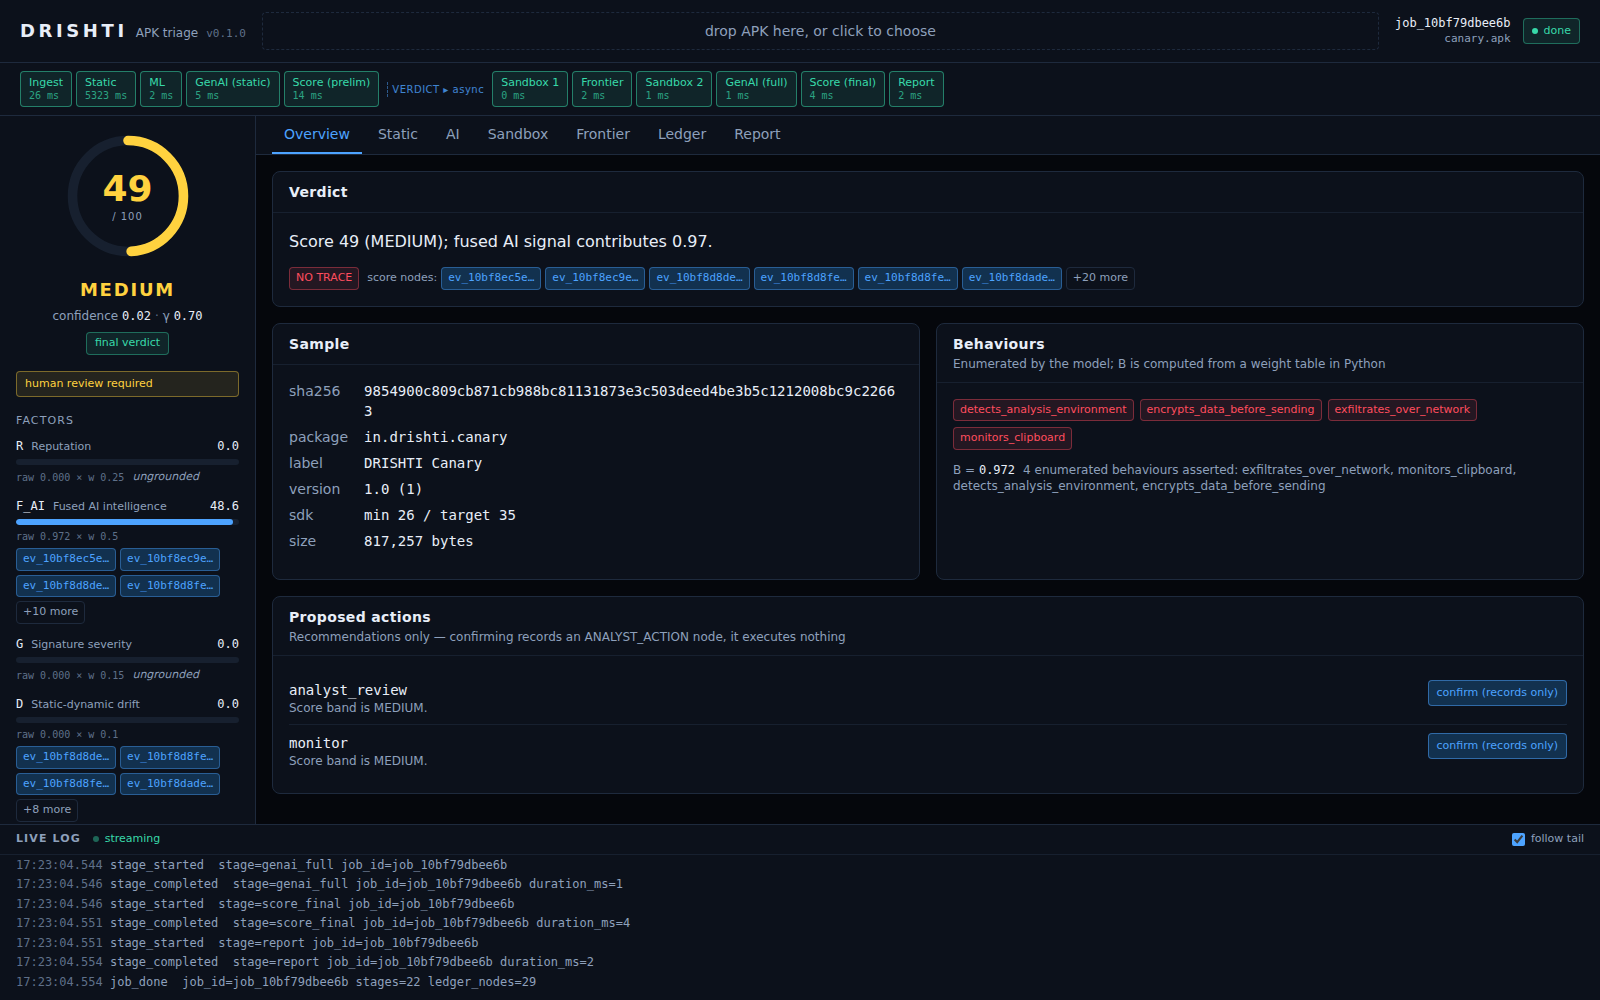
\includegraphics[width=\linewidth]{ui_overview.png}
\caption{The DRISHTI dashboard on a completed run
(\code{in.drishti.canary}, 22 stages, 29 ledger nodes). Left: the score
rail decomposing $\mathcal{S}$ into its four weighted factors. Centre: the
verdict, sample identity and enumerated behaviours. Bottom: the streaming
structured log. Note the elements that exist to \emph{limit} the claim, the red \textsc{no trace} provenance badge, the two factors labelled
\emph{ungrounded}, the \code{confidence 0.02} beside the score, and the
\code{human review required} flag.}
\label{fig:ui}
\end{figure*}
%=====================================================================
\section{Analyst Experience}
\label{sec:ux}
%=====================================================================

An analyst-facing tool earns trust in the interface or not at all. DRISHTI's
dashboard is therefore built on a single rule: \textbf{the screen never
asserts anything the ledger cannot substantiate, and it never hides the
weakness of its own evidence.} Figure~\ref{fig:ui} is a live run, no
mock-up, and almost every element on it exists to make a verdict
falsifiable rather than merely legible.


\subsection{The Score Is Audited on Screen, Not in a Paper}

The left rail does not present $\mathcal{S}=49$ as a number to be
accepted. It decomposes it into the four terms of
$\mathcal{S} = 0.25R + 0.50F_{\text{AI}} + 0.15G + 0.10D$ and shows the
arithmetic for each: \code{raw 0.972 $\times$ w 0.5} contributing 48.6 for
$F_{\text{AI}}$, and \code{raw 0.000 $\times$ w 0.25} for $R$. Crucially,
the two terms that contribute nothing are labelled \textbf{\emph{ungrounded}}
rather than left as a bare zero, the interface distinguishes ``we
looked and found nothing'' from ``we never looked,'' which is the
distinction on which an analyst's next action actually depends.

Every factor carries \textbf{evidence chips} (\code{ev\_10bf8ec5e…}) that
resolve to ledger nodes. A finding is never a claim in prose; it is one
click from the artefact that supports it. This is the evidence ledger of
Section~\ref{sec:ledger} surfaced as an interaction rather than a
compliance appendix.

\subsection{Honesty as an Interface Element}

Three affordances exist purely to prevent the system overselling itself:

\begin{itemize}
  \item \textbf{The provenance badge.} \textsc{no trace} in red states
        that nothing was detonated. It is derived from the trace's own
        image version, VM instance ID and timestamp, never from a
        configuration flag, so a replayed trace cannot be presented as
        a live one.
  \item \textbf{Confidence beside the score.} \code{confidence 0.02 ·
        $\gamma$ 0.70} sits next to \code{49 MEDIUM}. A high score with
        low confidence is displayed as exactly that, and because
        $\gamma$ is structurally capped without detonation, the interface
        is incapable of showing false certainty.
  \item \textbf{Enumerated behaviours, not prose.} The behaviours panel
        states in the interface itself that ``\emph{B} is computed from a
        weight table in Python,'' and lists the four booleans the model
        asserted. A judge, or an auditor, can see that the model
        named behaviours and did not choose a number.
\end{itemize}

\subsection{Preliminary Verdict First, Depth Asynchronously}

The stage strip renders the pipeline as it executes and makes the
system's central latency decision visible: stages up to
\code{Score (prelim)} complete in \textbf{under 5.4\,s}, at which point
the strip shows an explicit \code{VERDICT $\blacktriangleright$ async}
divider and the analyst already has an actionable band. The sandbox,
frontier and full-GenAI stages continue behind that verdict and revise it
when they finish. An analyst is never blocked on the slowest component,
and the streaming structured log at the foot of the screen means a
long-running job is legible while it runs rather than opaque until it
ends.

\subsection{Human-in-the-Loop, Enforced in the Product}

The \emph{Proposed actions} panel recommends \code{analyst\_review} and
\code{monitor}, and states plainly beneath the heading:
``\emph{Recommendations only, confirming records an
\code{ANALYST\_ACTION} node, it executes nothing.}'' Confirmation writes a
signed node to the ledger; it does not block a URL, notify a customer, or
push an IOC. DRISHTI is decision-support by construction, and the
interface is where that guarantee is made legible to the person
accountable for the decision.

\subsection{Workflow Depth}

Seven tabs follow the analyst's escalation path rather than the system's
module boundaries, \textsc{overview} for the verdict,
\textsc{static}, \textsc{ai}, \textsc{sandbox} and \textsc{frontier} for
the layer that produced a given finding, \textsc{ledger} for the full
hash chain with one-click verification, and \textsc{report} for the
exportable artefact. Panels that depend on unbuilt modules render an
explicit \emph{not yet implemented} state naming the owning task, rather
than an empty panel or a plausible placeholder. Even the absence of a
feature is reported honestly.

%=====================================================================
\section{Conclusion}
\label{sec:conclusion}
%=====================================================================

DRISHTI addresses the full spectrum of APK-borne financial fraud:
Level~1 malicious artefacts detectable by static and ML analysis, and
the harder Level~2 latent threats that evade every existing scanner.
Its core innovation is a GenAI reasoning layer that does not merely
classify - it acts as an automated reverse engineer, synthesising the
very environment a dormant trojan is hunting for to make it confess,
then binding every sentence of its verdict to a concrete artefact that
an analyst can verify.

The evidence ledger transforms AI output from an opaque score into a
machine-generated audit trail. The GenAI-synthesised sandbox - emulating
dead C2 infrastructure and morphing device state Just-in-Time - unrolls
behaviour that dormant trojans conceal from generic sandboxes. The
multi-label ML ensemble provides signature-agnostic generic checks and
calibrates confidence. GenAI reverse engineering exposes the malware's
intent, impersonated target, and victim demographic. Together, these
layers deliver what bank fraud desks actually need: not ``this looks
malicious'' but ``here is exactly what this app does, here is the
proof, here is the YARA rule to find its siblings, and here is who it
targets.''

\begin{principlebox}[The DRISHTI thesis]
GenAI is a first-class analyst inside the detection pipeline - reading
decompiled code and live behaviour the way a human reverse engineer
would, and actively synthesising the conditions that force malware to
reveal itself - while the threat score is produced by a calibrated,
explainable, multi-signal engine. Every verdict is bound to
cryptographic evidence, and a human confirms every consequential action.
The AI reasons; it never guesses the number.
\end{principlebox}

\vspace{4pt}
Every other system classifies an APK. \textbf{DRISHTI interrogates it.}

%=====================================================================
%=====================================================================

{\scriptsize
\begin{thebibliography}{99}
\setlength{\itemsep}{1pt}

\bibitem{vt_insight}
  VirusTotal.
  \textit{Introducing VirusTotal Code Insight: Empowering threat analysis with generative AI.}
  \url{https://blog.virustotal.com/2023/04/introducing-virustotal-code-insight.html}

\bibitem{vt_ai}
  VirusTotal.
  \textit{Empowering Defenders: How AI is shaping malware analysis.}
  \url{https://assets.virustotal.com/reports/2023-ai}

\bibitem{sysdig_genai}
  Sysdig.
  \textit{More than an Assistant - A New Architecture for GenAI in Cloud Security.}
  \url{https://www.sysdig.com/blog/genai-cloud-security}

\bibitem{sysdig_sage}
  Sysdig.
  \textit{Sysdig Sage: A groundbreaking AI security analyst.}
  \url{https://www.sysdig.com/blog/sysdig-sage-a-groundbreaking-ai-security-analyst}

\bibitem{sysdig_falco}
  Sysdig.
  \textit{What is Falco? Open source runtime threat detection.}
  \url{https://www.sysdig.com/learn-cloud-native/what-is-falco}

\bibitem{rbi2024}
  Reserve Bank of India.
  \textit{Annual Report on Cyber Security in the Indian Banking Sector, 2024.}
  \url{https://www.rbi.org.in}

\bibitem{mitre_mobile}
  MITRE.
  \textit{ATT\&CK for Mobile.}
  \url{https://attack.mitre.org/matrices/mobile/}

\bibitem{mobsf}
  Mobile Security Framework (MobSF).
  \url{https://github.com/MobSF/Mobile-Security-Framework-MobSF}

\bibitem{frida}
  Frida - Dynamic instrumentation toolkit.
  \url{https://frida.re/}

\bibitem{androguard}
  Androguard.
  \url{https://github.com/androguard/androguard}

\bibitem{yara}
  YARA.
  \url{https://virustotal.github.io/yara/}

\bibitem{abusech}
  abuse.ch - MalwareBazaar \& URLhaus.
  \url{https://abuse.ch/}

\bibitem{androzoo}
  AndroZoo dataset.
  \url{https://androzoo.uni.lu/}

\bibitem{cicmaldroid}
  CIC-MalDroid 2020.
  \url{https://www.unb.ca/cic/datasets/maldroid-2020.html}

\bibitem{quark}
  Quark-Engine.
  \url{https://github.com/quark-project/quark-engine}

\bibitem{repo}
  Team DRISHTI. \textit{CyberShield / DRISHTI, prototype implementation.}
  \url{https://github.com/Soni-Shivam/CyberShield}

\end{thebibliography}
}

\end{document}